\documentclass[12pt, twoside]{article}
\usepackage[francais]{babel}
\usepackage[T1]{fontenc}
\usepackage[latin1]{inputenc}
\usepackage[left=5mm, right=5mm, top=5mm, bottom=5mm]{geometry}
\usepackage{float}
\usepackage{graphicx}
\usepackage{array}
\usepackage{multirow}
\usepackage{amsmath,amssymb,mathrsfs} 
\usepackage{soul}
\usepackage{textcomp}
\usepackage{eurosym}
\usepackage{lscape}
 \usepackage{variations}
\usepackage{tabvar}
 
\pagestyle{empty}


\date{}

\begin{document}

\enskip


\begin{center}
\Large{\ul{\textbf{Configuration de Thal�s}}}
\end{center}

\vspace{1cm}

\fbox{
\begin{minipage}{18cm}
\ul{Th�or�me de Thal�s}: 

\enskip


\begin{enumerate}
  \item [$\bullet$](d) et (d') sont deux droites s�cantes en A.
  \item  [$\bullet$] B et M sont deux points de (d) distincts de A.
  \item [$\bullet$] C et N sont deux points de (d') distincts de A.
\end{enumerate}


\enskip

\qquad \qquad Si les droites (BC) et (MN) sont parall�les alors
$\dfrac{AM}{AB}=\dfrac{AN}{AC}=\dfrac{MN}{BC}$


\quad 
\end{minipage}
}


\bigskip


\ul{Figures-cl�s}:


\begin{tabular}{ccc}
\begin{minipage}{6cm}
\begin{center}
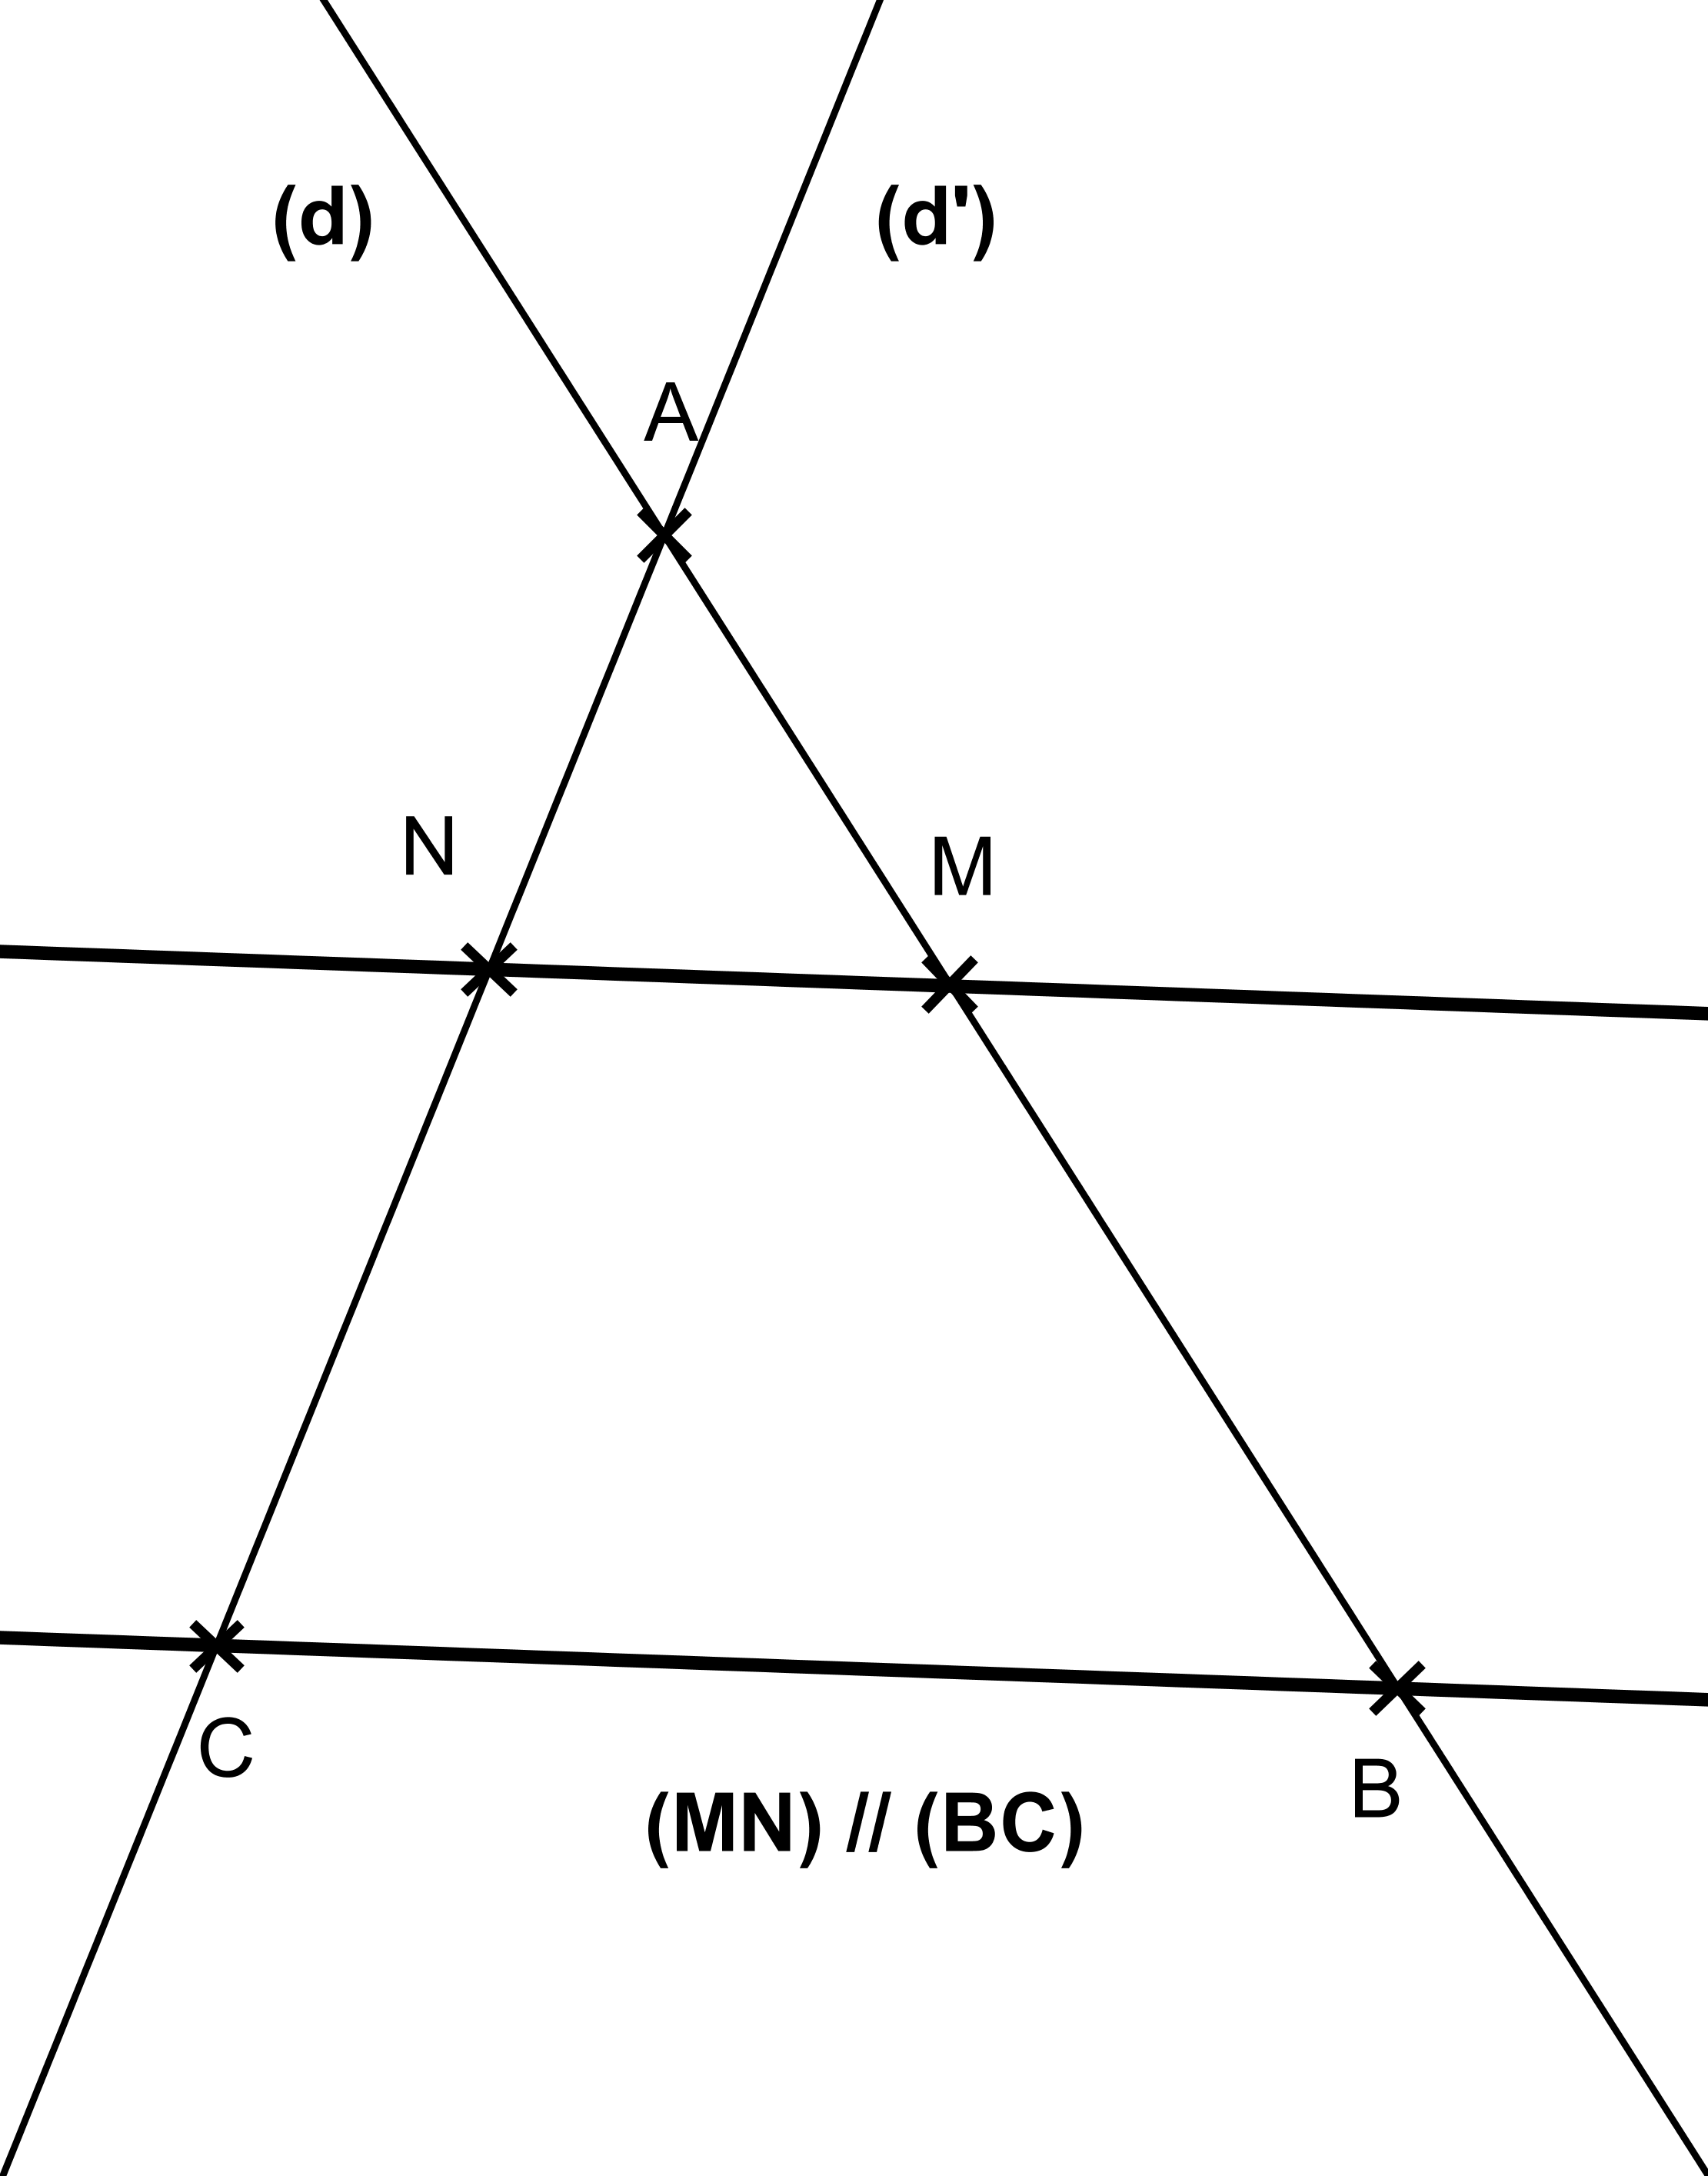
\includegraphics[width=5cm]{images/ex1.png}
\end{center}
\end{minipage}
&
\begin{minipage}{6cm}
\begin{center}
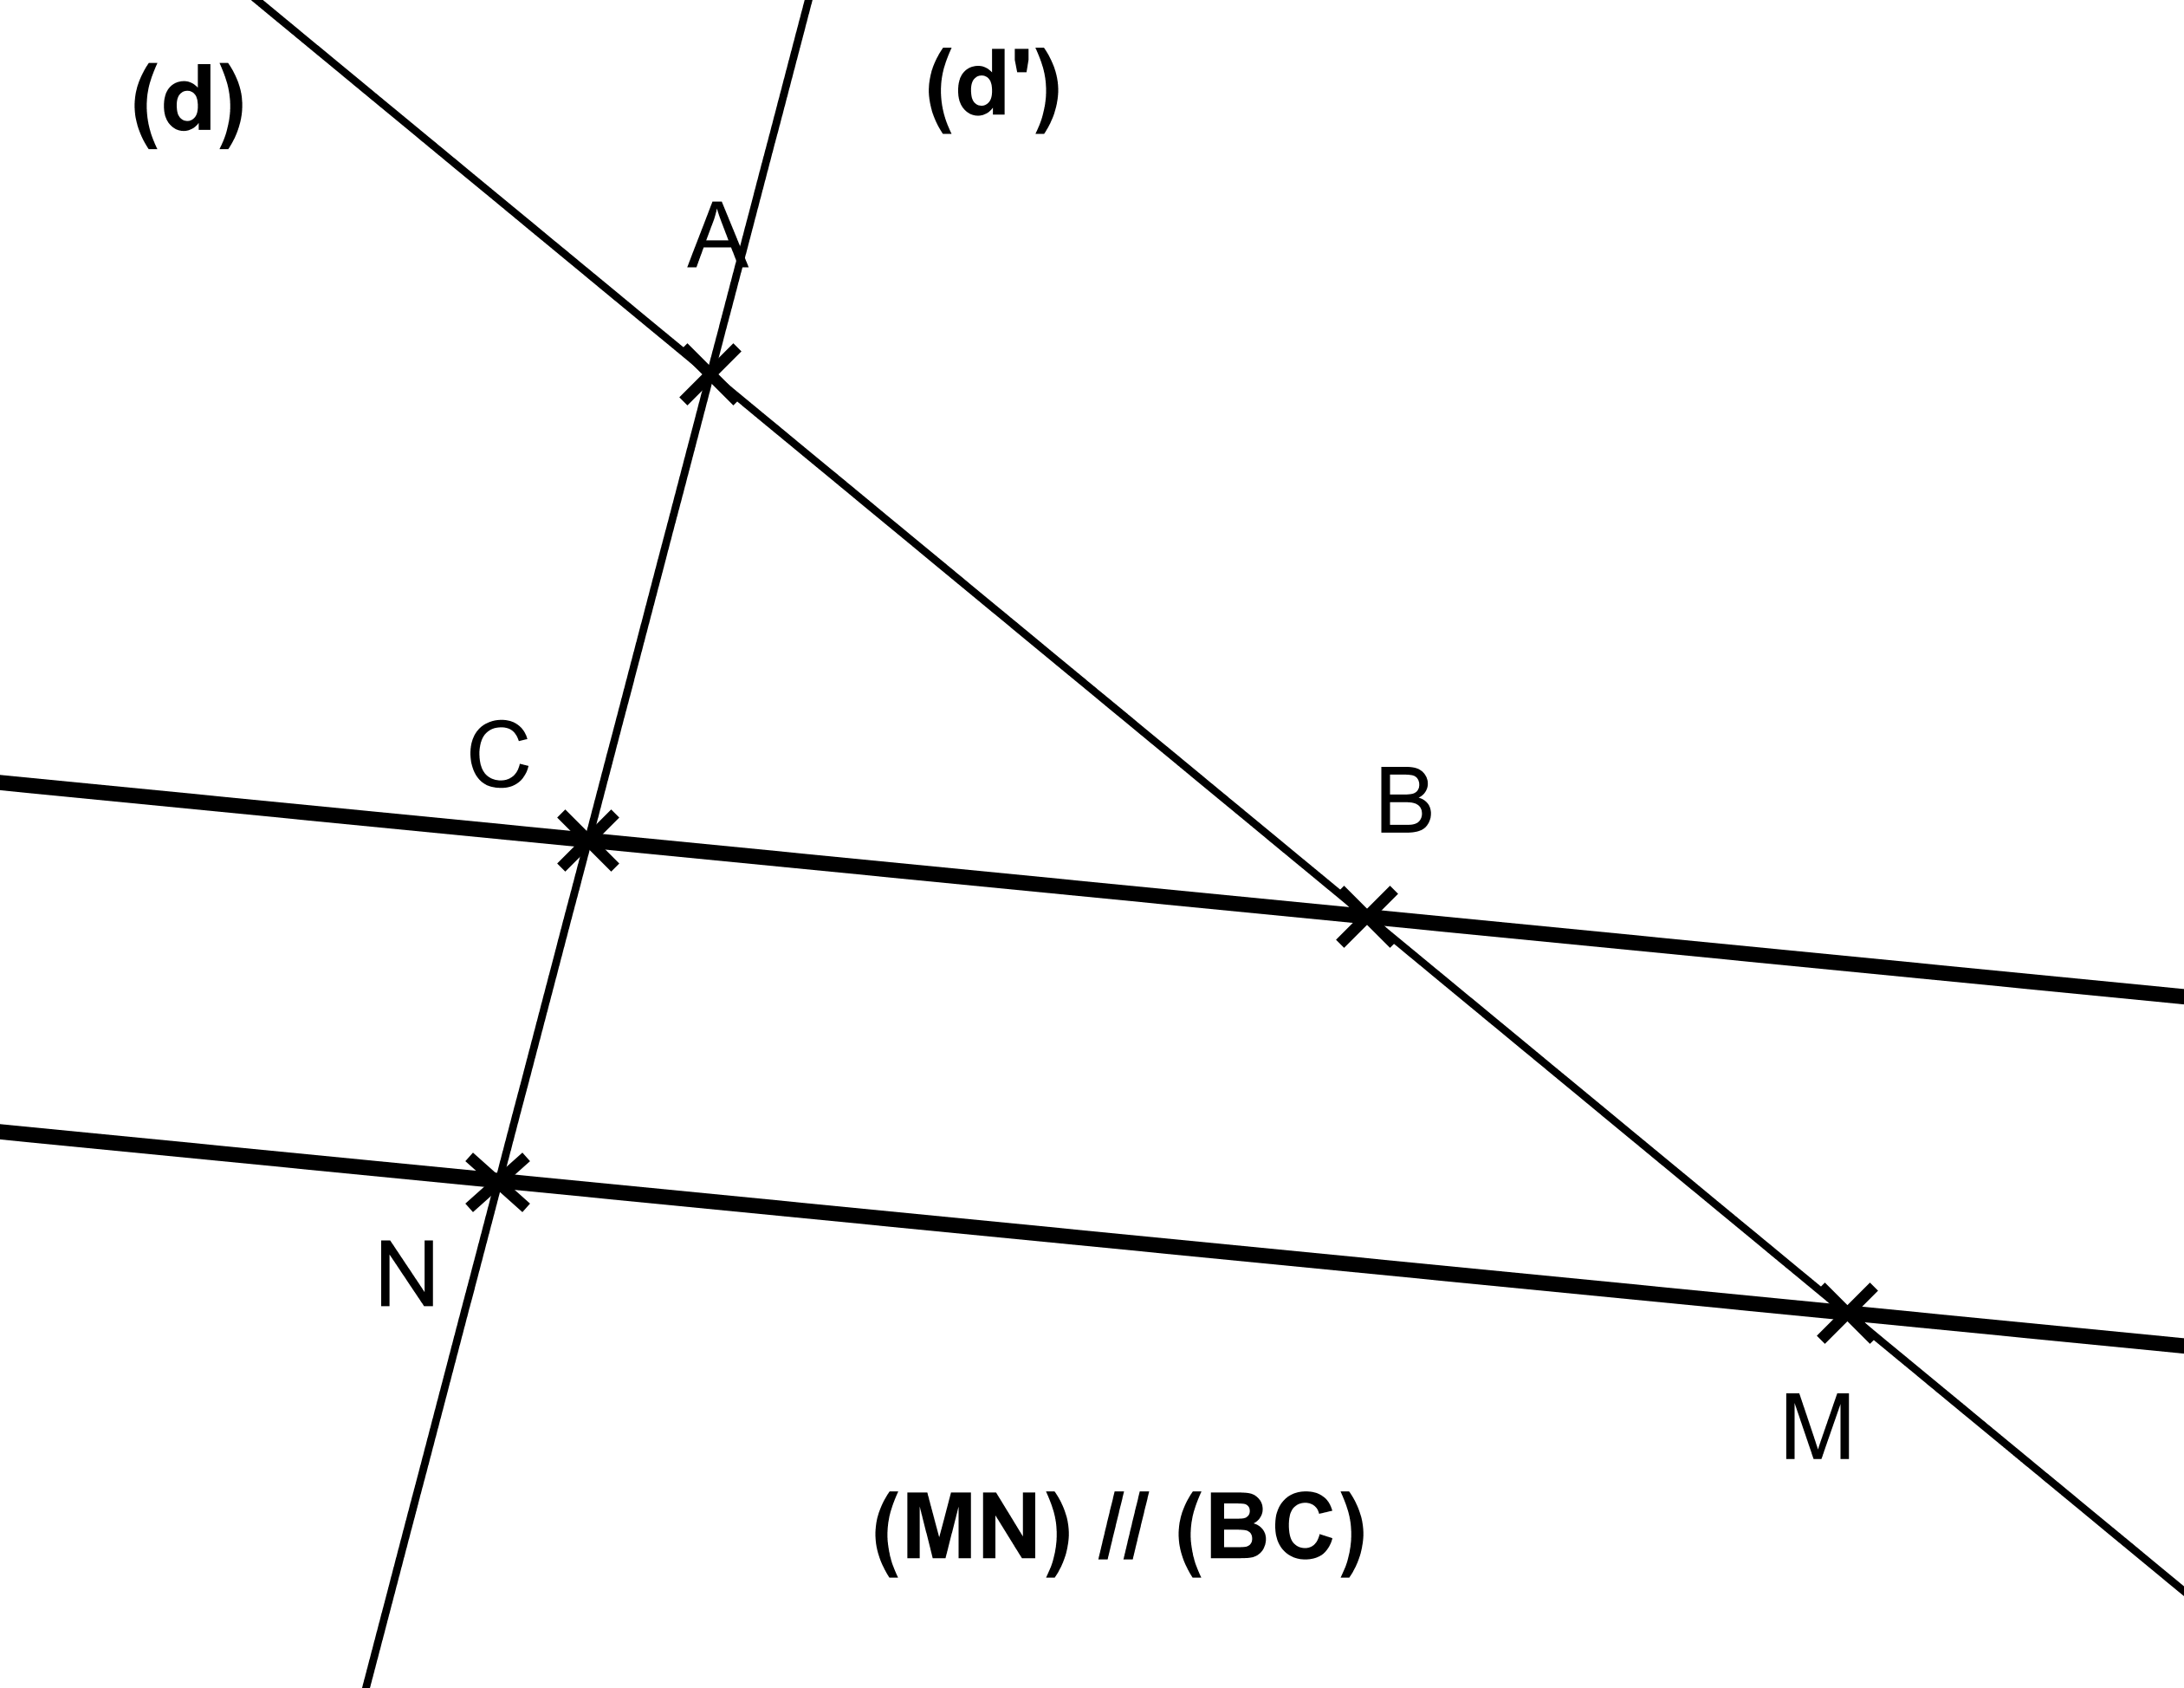
\includegraphics[width=5cm]{images/ex2.png}
\end{center}
\end{minipage}
& 
\begin{minipage}{6cm}
\begin{center}
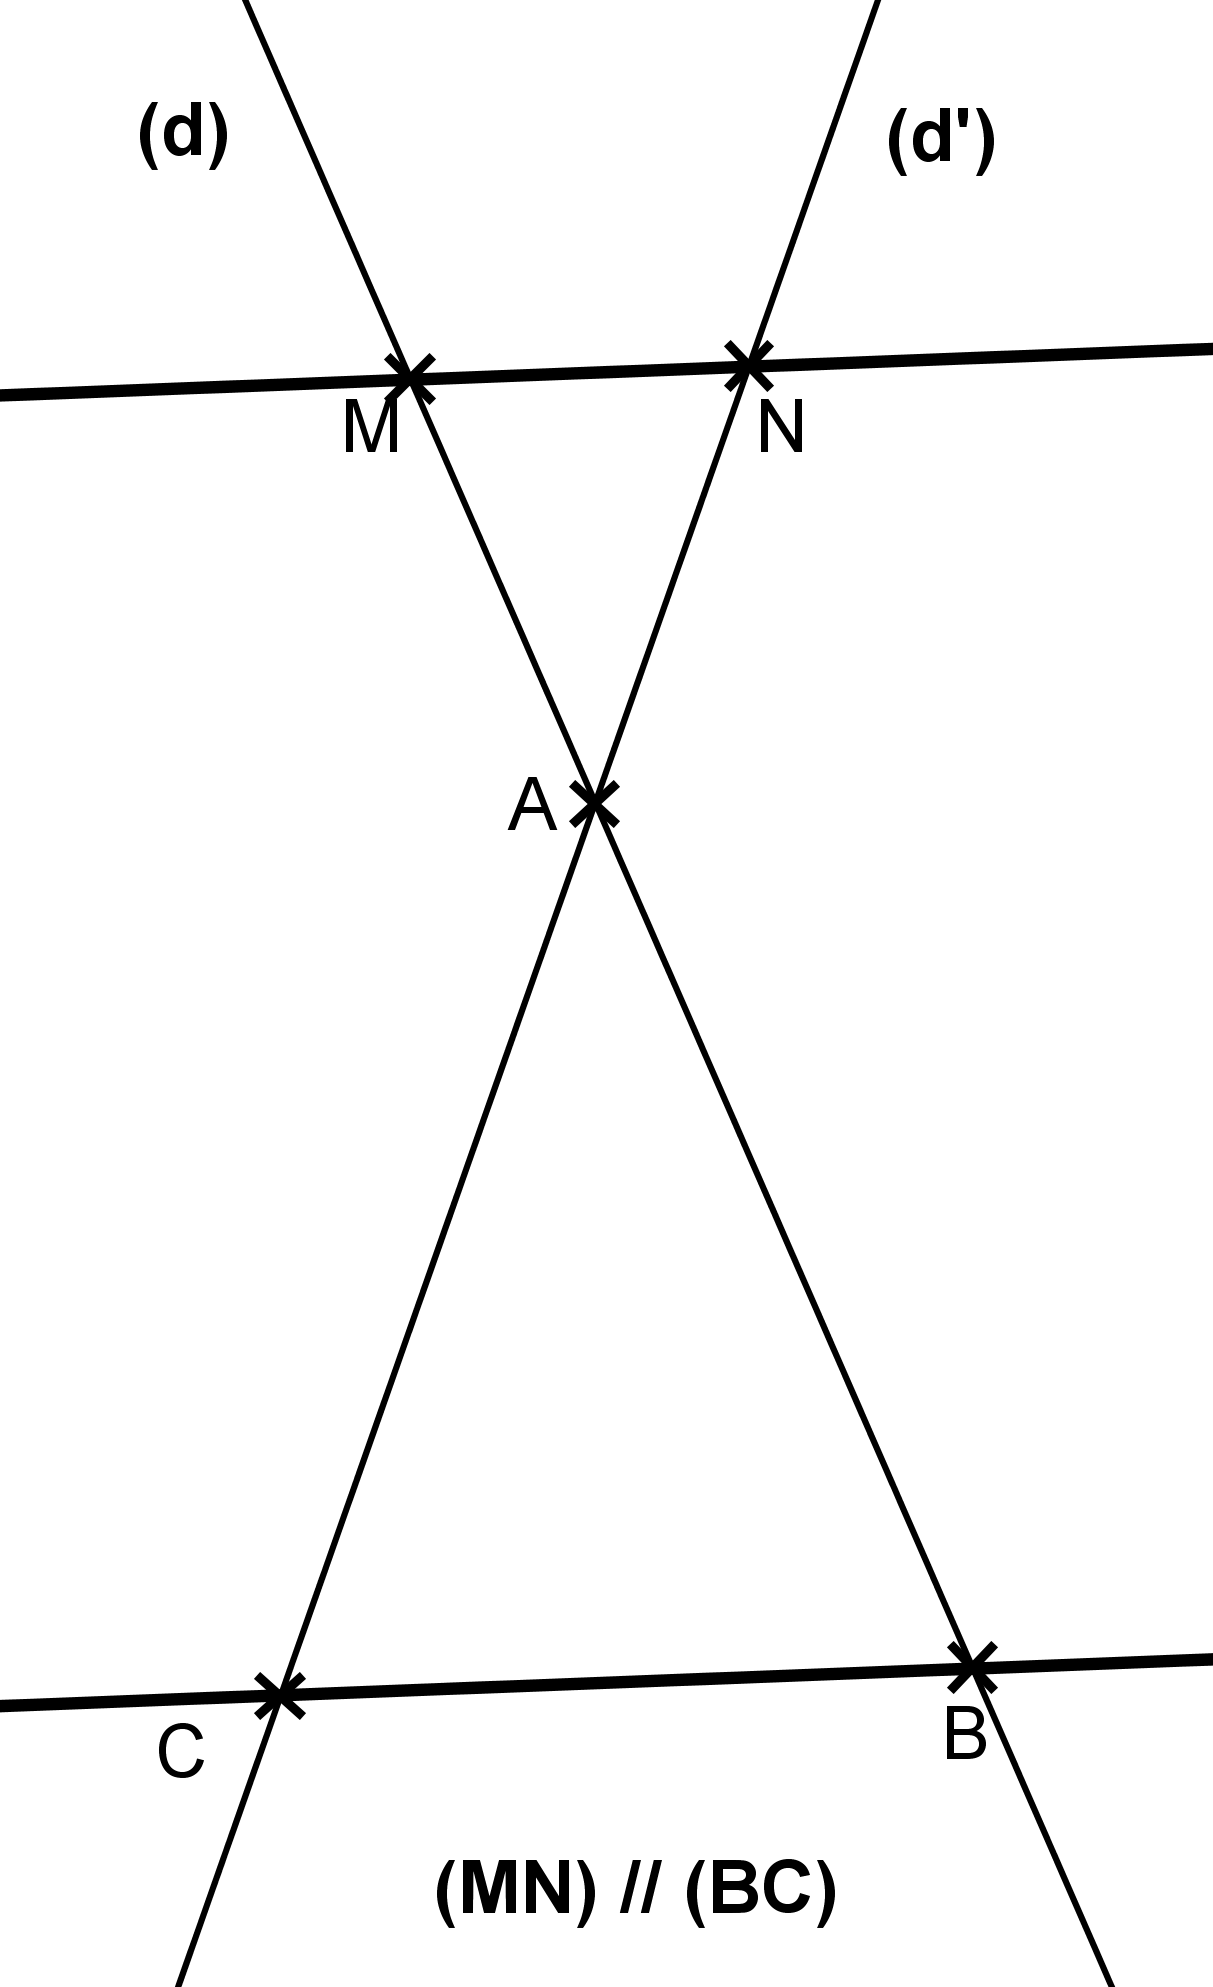
\includegraphics[width=4cm]{images/ex3.png}
\end{center}
\end{minipage}
\end{tabular}

\enskip


\begin{center}
alors \quad $\dfrac{AM}{AB}=\dfrac{AN}{AC}=\dfrac{MN}{BC}$
\end{center}



\bigskip


\ul{Remarque}: 
 Le tableau suivant est un tableau de proportionnalit�:


\begin{center}
\begin{tabular}{|c|c|c|c|}
\hline
longueurs des cot�s du triangle AMN & \qquad \qquad & \qquad \qquad & \qquad
\qquad
\\

\hline
longueurs des cot�s du triangle ABC & \qquad \qquad & \qquad \qquad & \qquad
\qquad
\\

\hline
\end{tabular}
\end{center}




\bigskip


\ul{M�thode pour calculer des longueurs}:

\enskip


\begin{tabular}{cc}
\begin{minipage}{12cm}
Sur la figure ci-contre, les droites (LM) et (JK) sont parall�les et les
droites (LK) et (MJ) sont s�cantes en I. On donne LI=4cm, IM=5cm, IK=6cm et
JK=10,5cm. Calculer les longueurs IJ et ML.

\end{minipage}
&
\begin{minipage}{6cm}
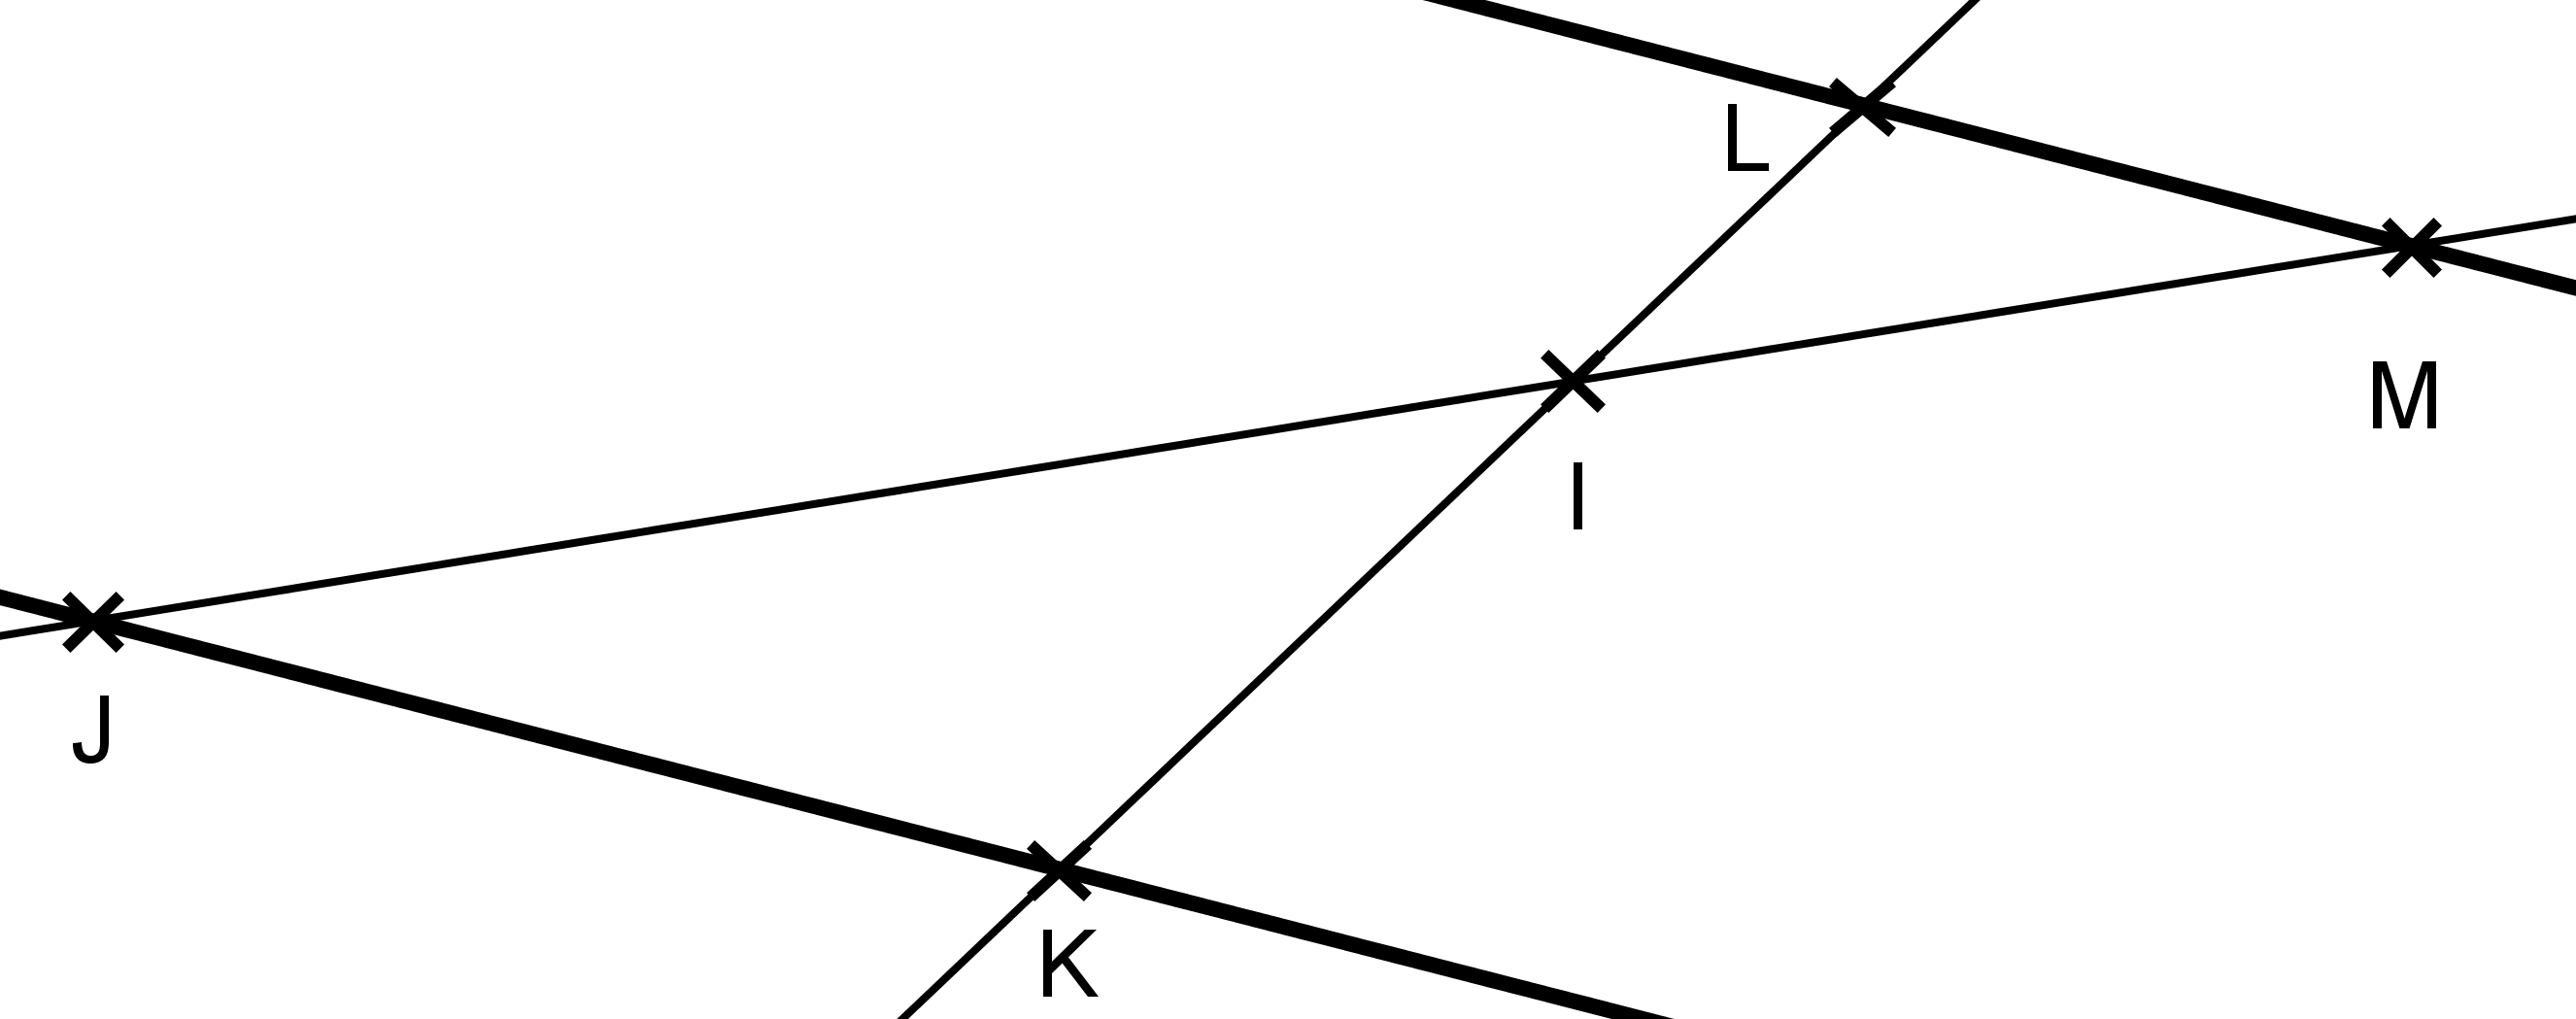
\includegraphics[width=6cm]{images/exemple.png}
\end{minipage}
\end{tabular}  

\enskip


Les droites (LK) et (MJ) sont s�cantes en I. Les droites (LM) et (JK) sont
parall�les. Donc d'apr�s le th�or�me de Thal�s, on a:
$\dfrac{IM}{IJ}=\dfrac{IL}{IK}=\dfrac{ML}{JK}$.


En rempla�ant par les valeurs num�riques:
$\dfrac{5}{IJ}=\dfrac{4}{6}=\dfrac{ML}{10,5}$


\enskip

\textbf{Calcul de IJ:} $\dfrac{5}{IJ}=\dfrac{4}{6}$
\qquad L'�galit� des produits en croix donne: $IJ=\dfrac{5 \times 6}{4}=7,5$cm.


\enskip

\textbf{Calcul de ML:} $\dfrac{4}{6}=\dfrac{ML}{10,5}$ \qquad 
L'�galit� des produits en croix donne: $ML=\dfrac{10,5 \times 4}{6}=7$cm.


\pagebreak

\vspace{2cm}


\ul{Figures-cl�s}:


\begin{tabular}{ccc}
\begin{minipage}{6cm}
\begin{center}
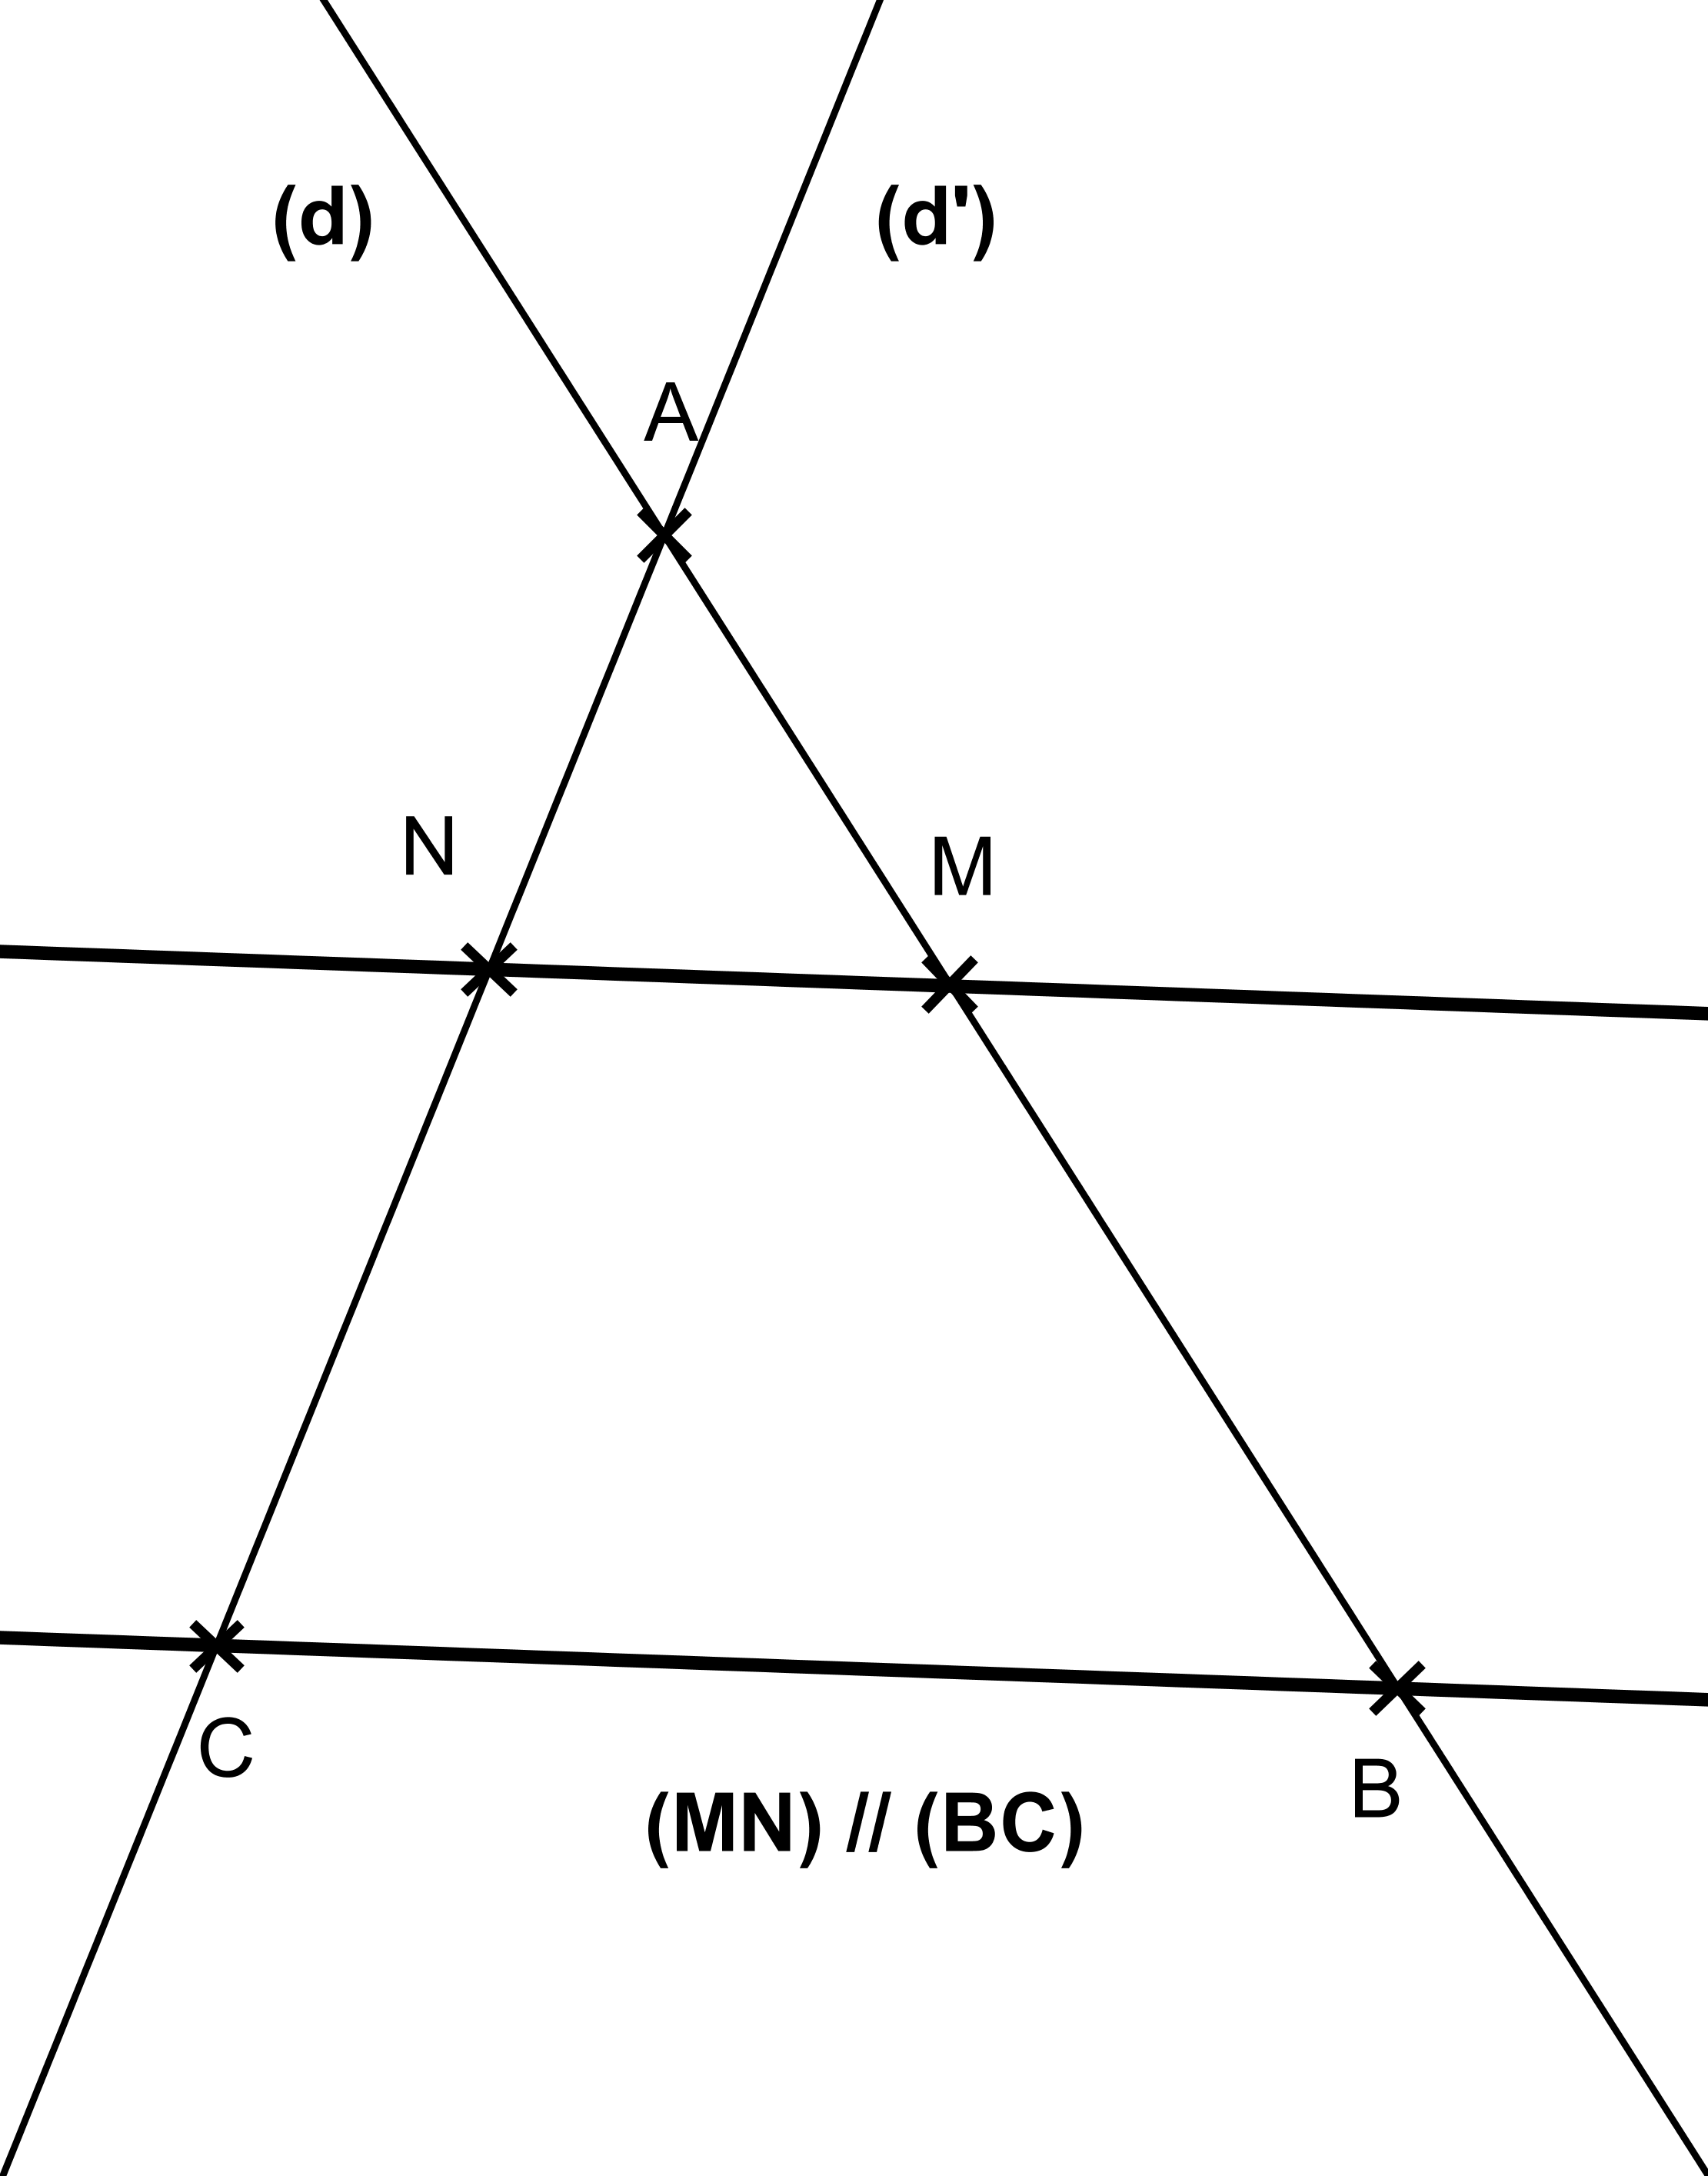
\includegraphics[width=5cm]{images/ex1.png}
\end{center}
\end{minipage}
&
\begin{minipage}{6cm}
\begin{center}
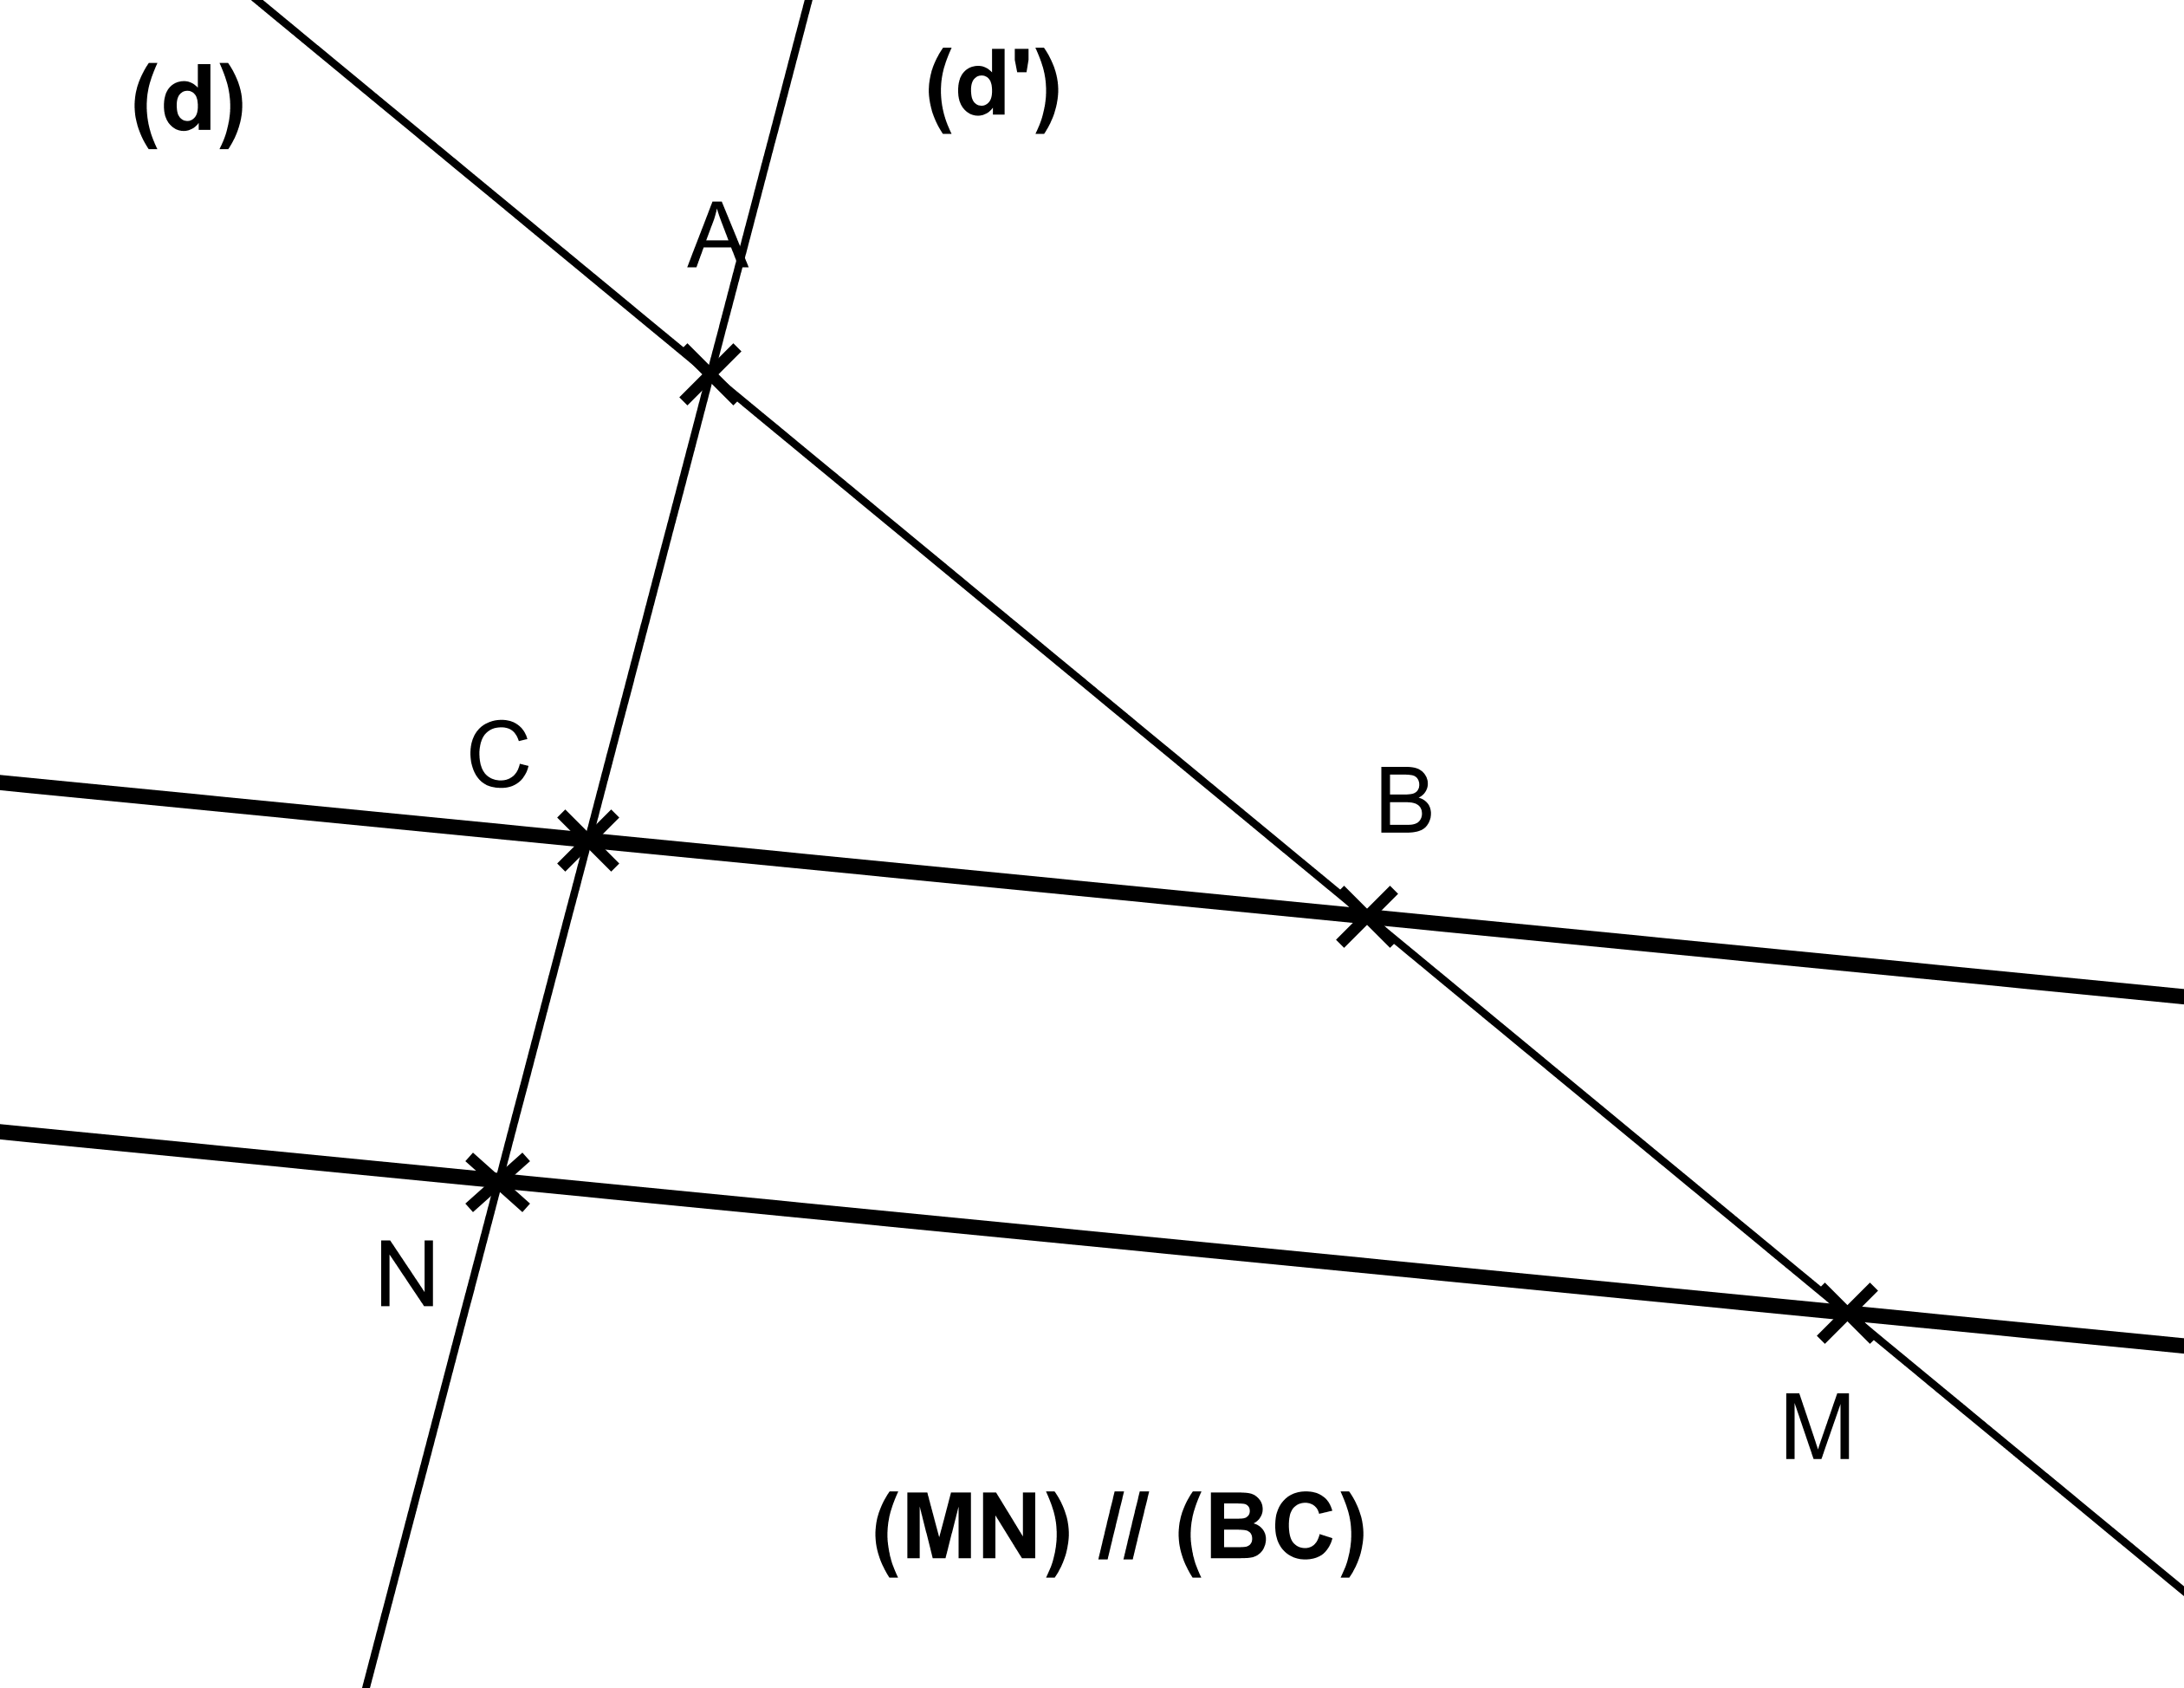
\includegraphics[width=5cm]{images/ex2.png}
\end{center}
\end{minipage}
& 
\begin{minipage}{6cm}
\begin{center}
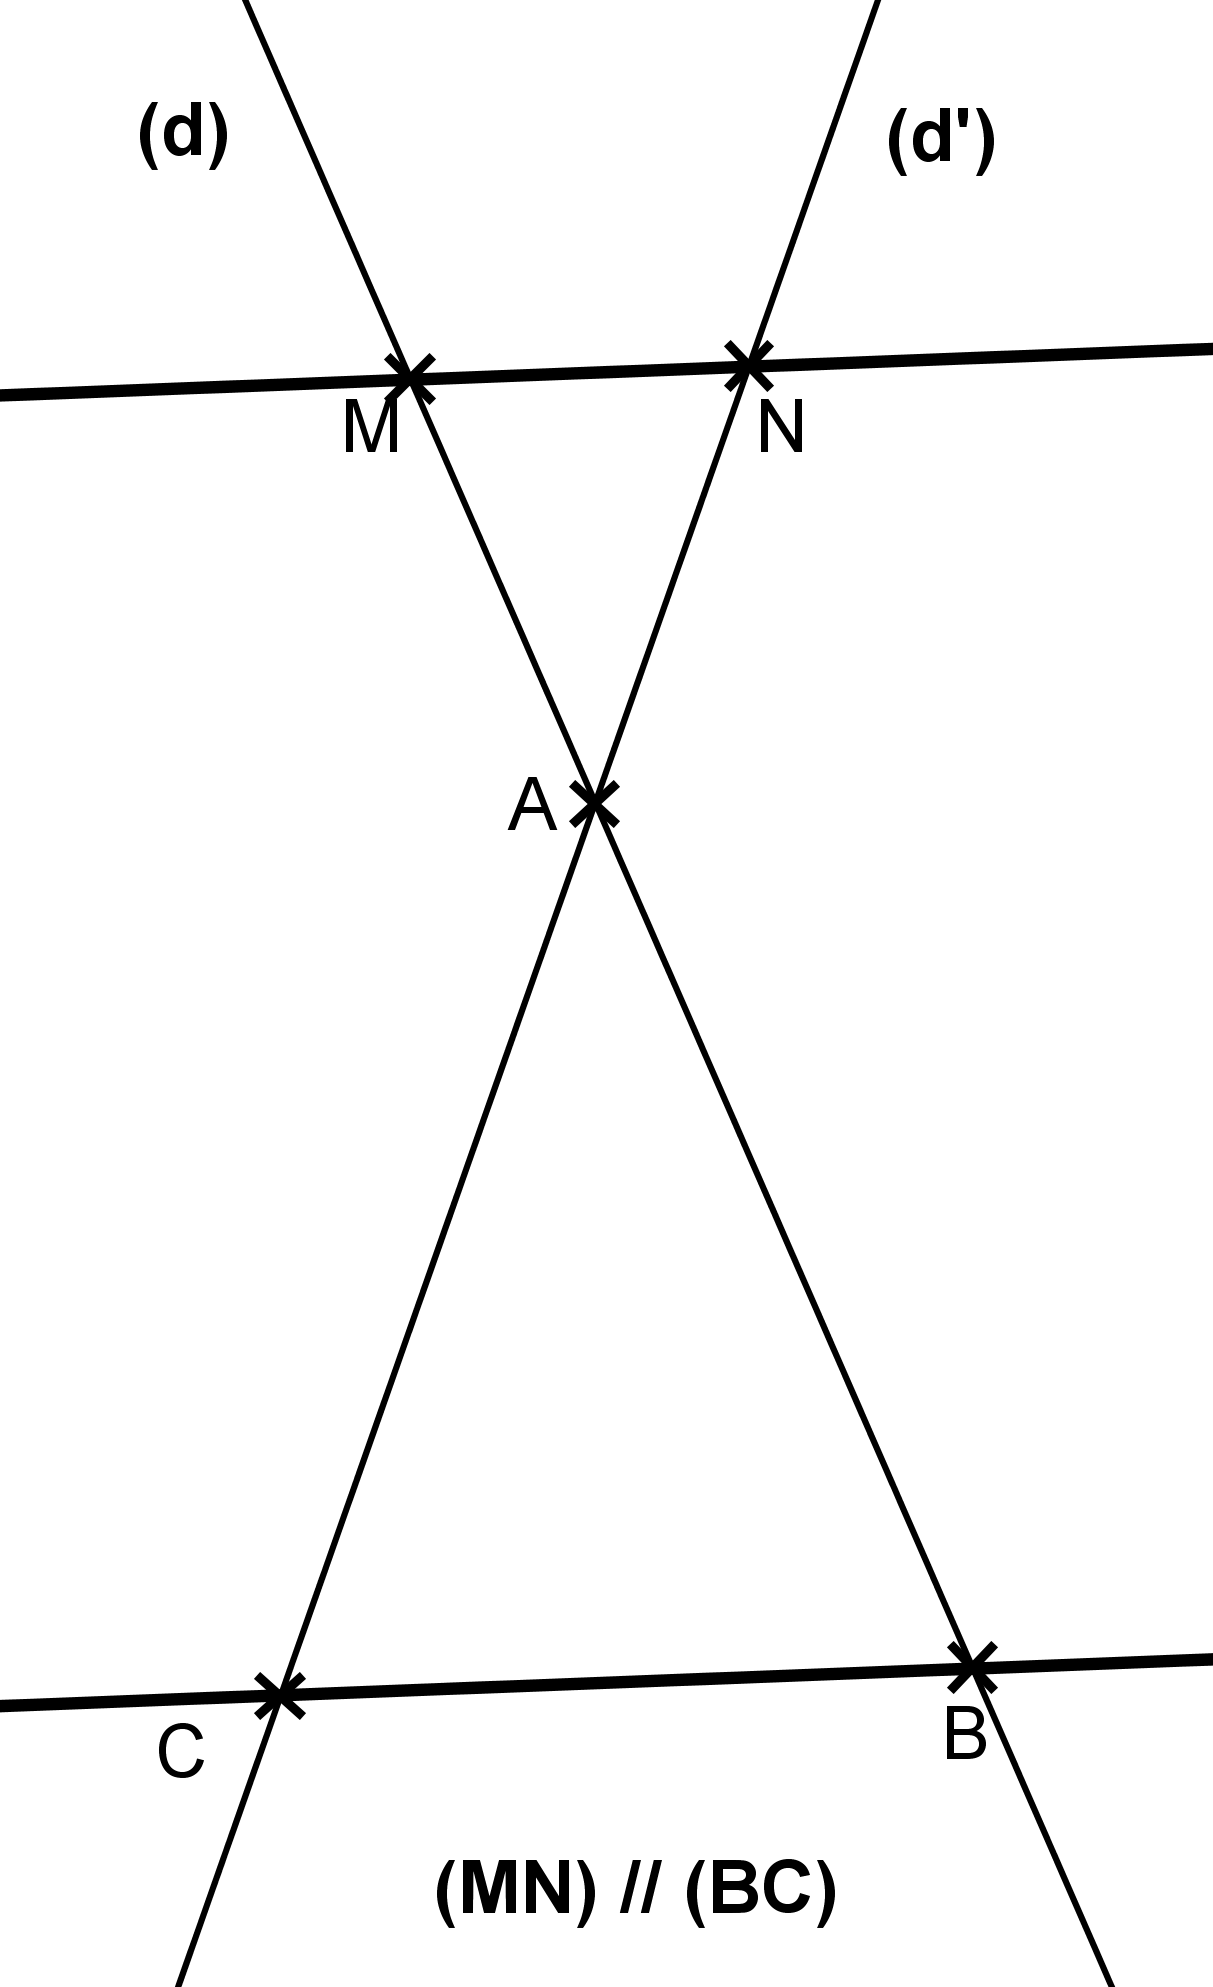
\includegraphics[width=4cm]{images/ex3.png}
\end{center}
\end{minipage}
\end{tabular}


\vspace{2cm}

\ul{Figures-cl�s}:


\begin{tabular}{ccc}
\begin{minipage}{6cm} 
\begin{center}
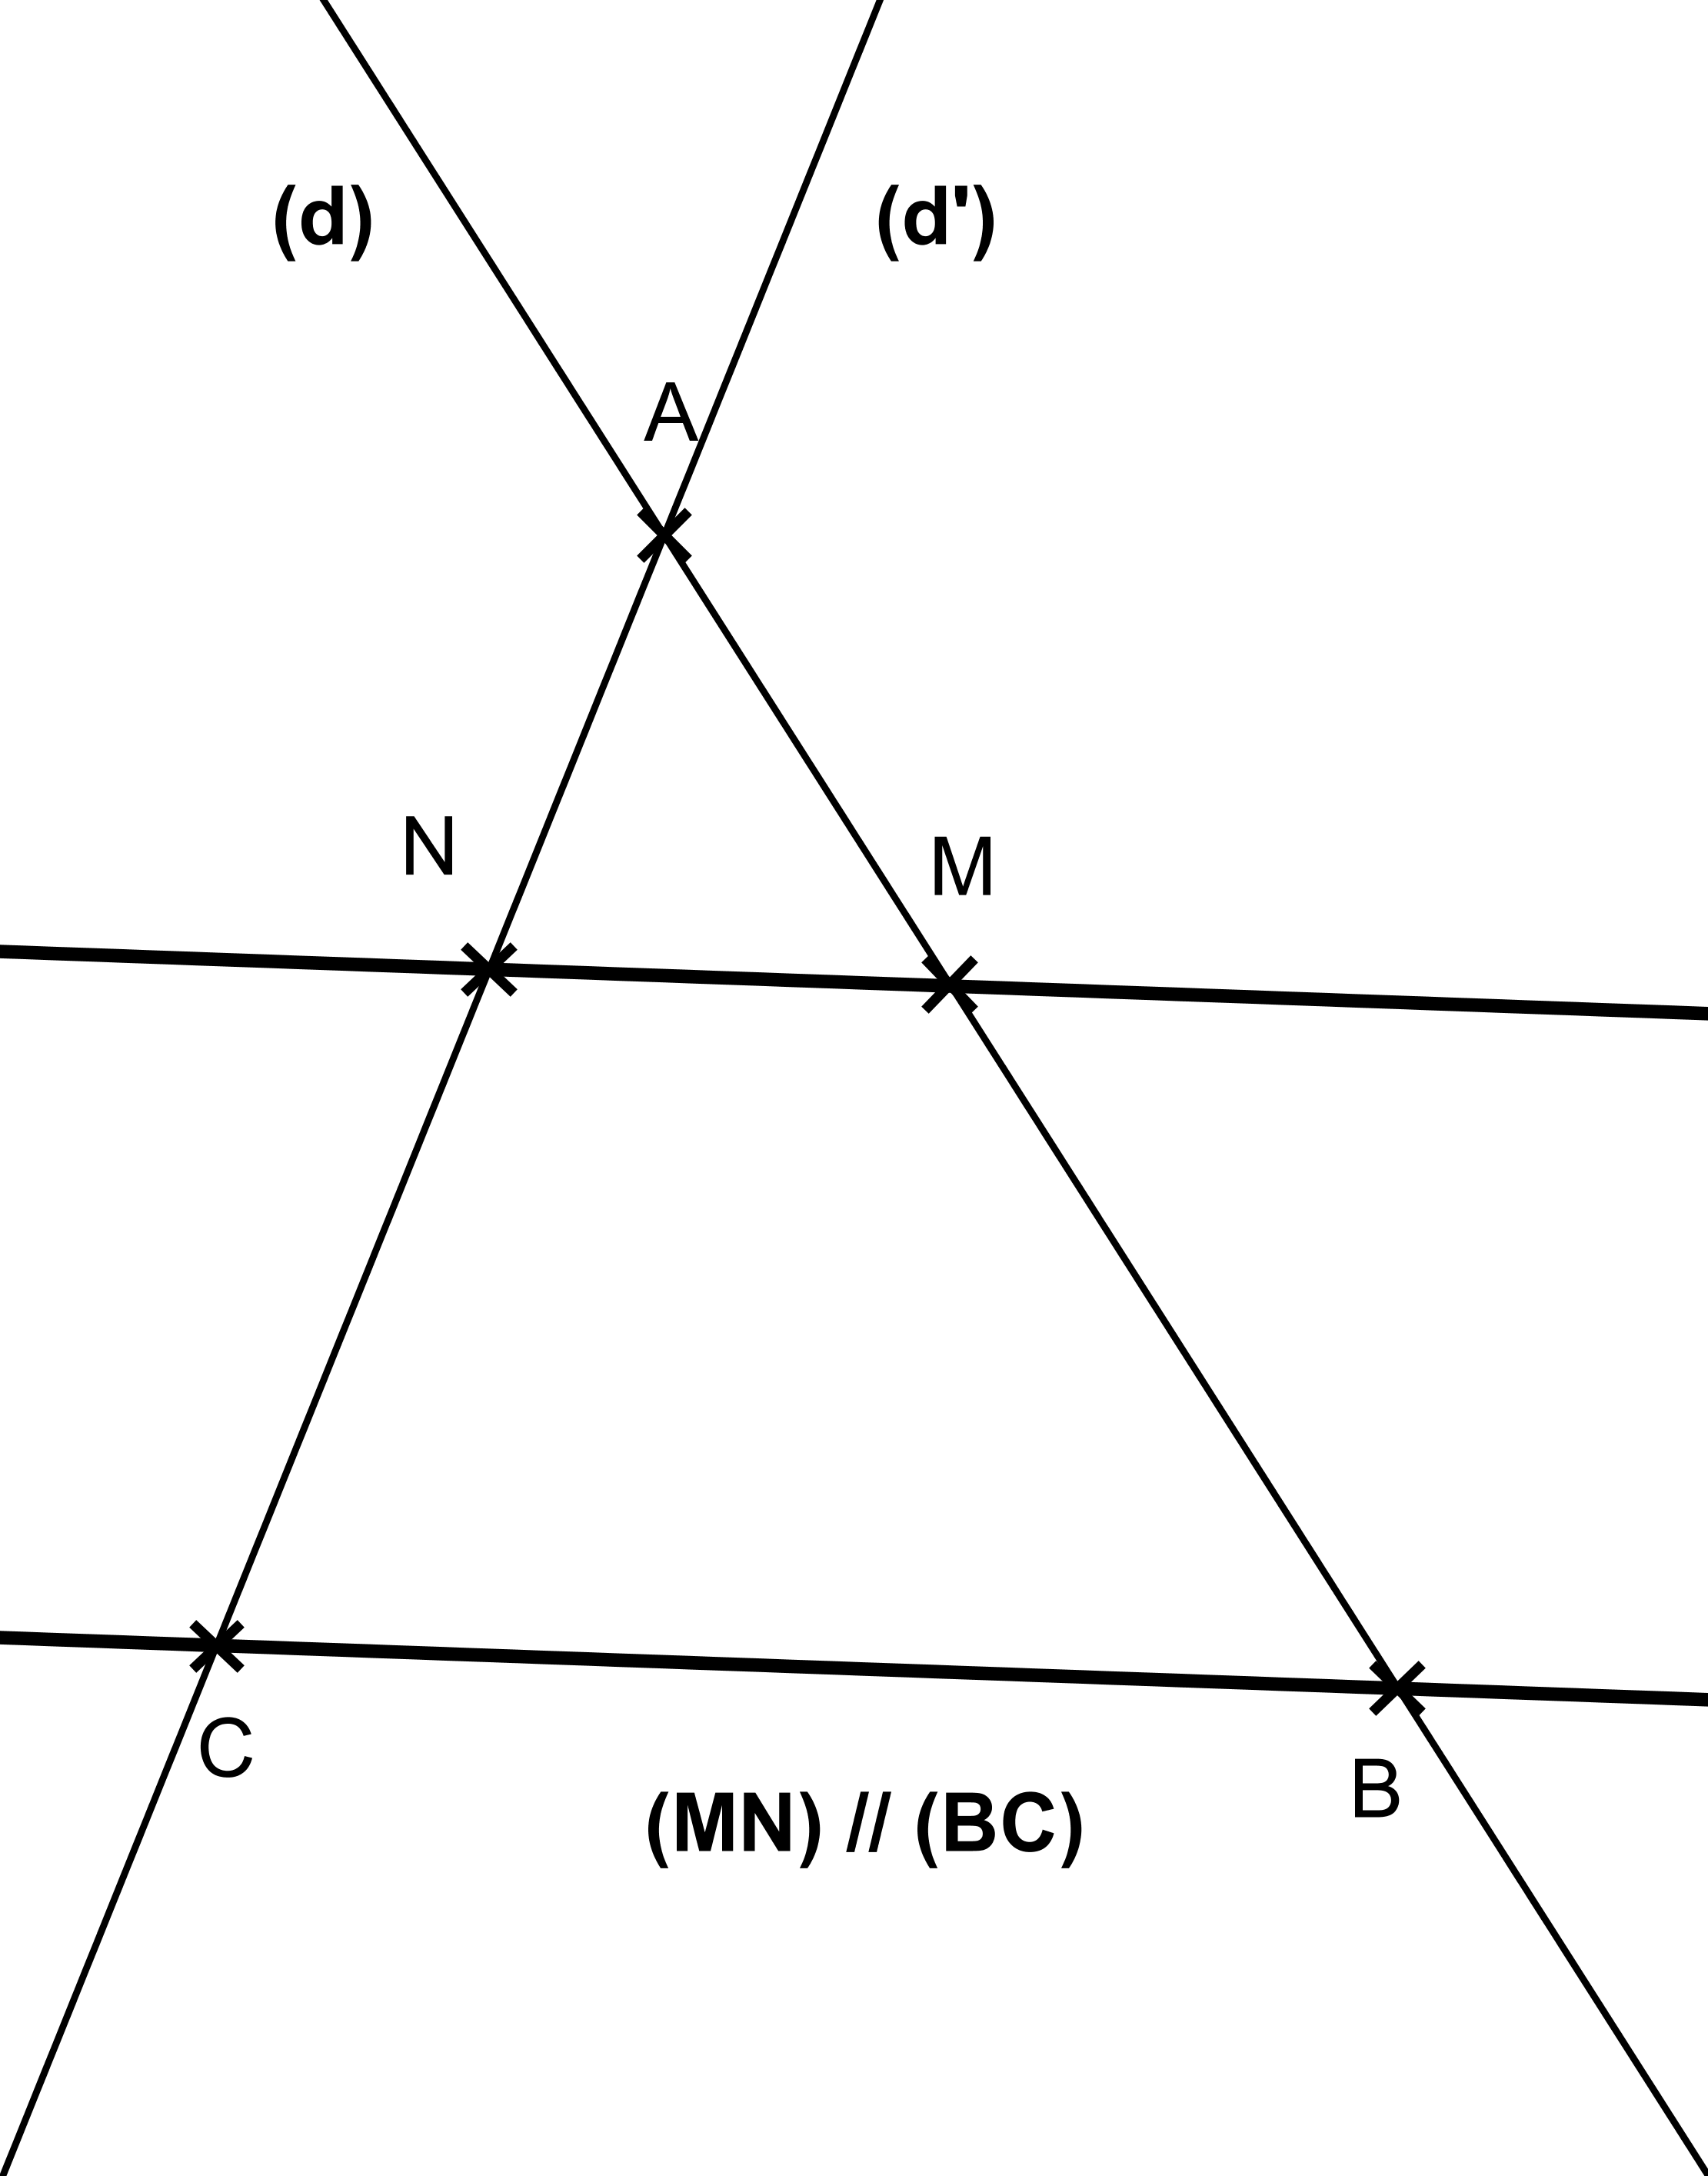
\includegraphics[width=5cm]{images/ex1.png}
\end{center}
\end{minipage}
&
\begin{minipage}{6cm}
\begin{center}
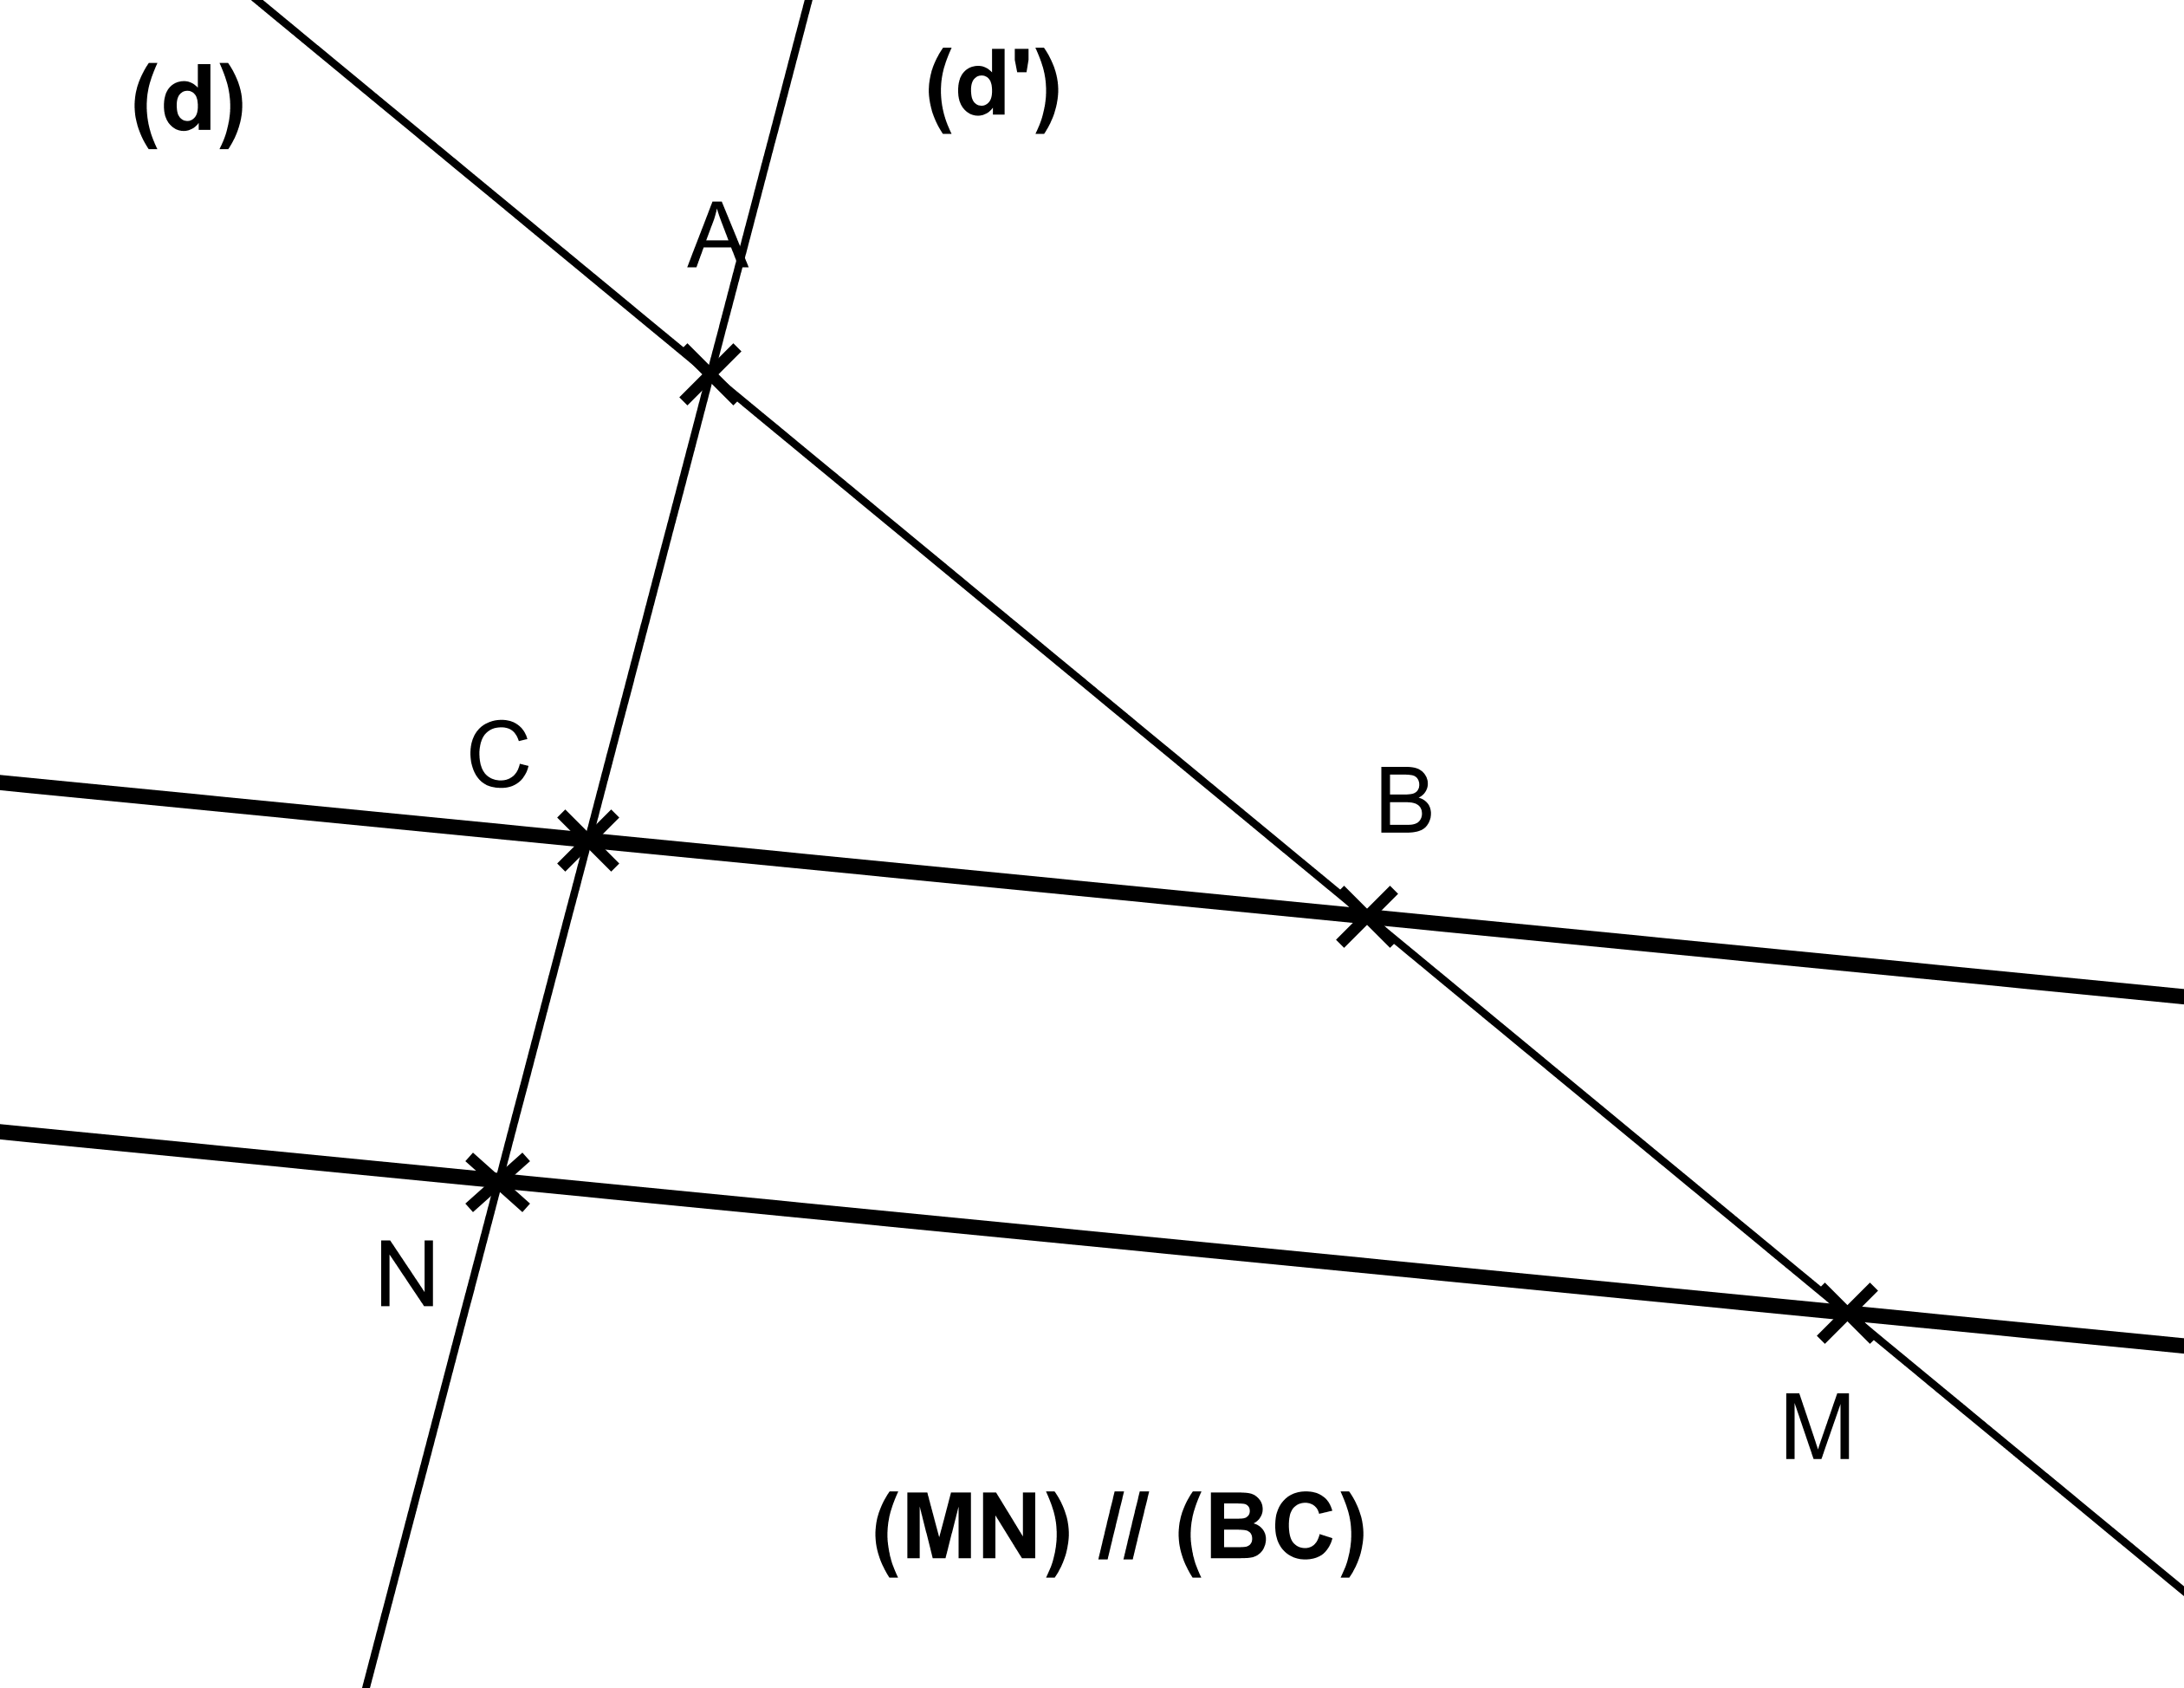
\includegraphics[width=5cm]{images/ex2.png}
\end{center}
\end{minipage}
& 
\begin{minipage}{6cm}
\begin{center}
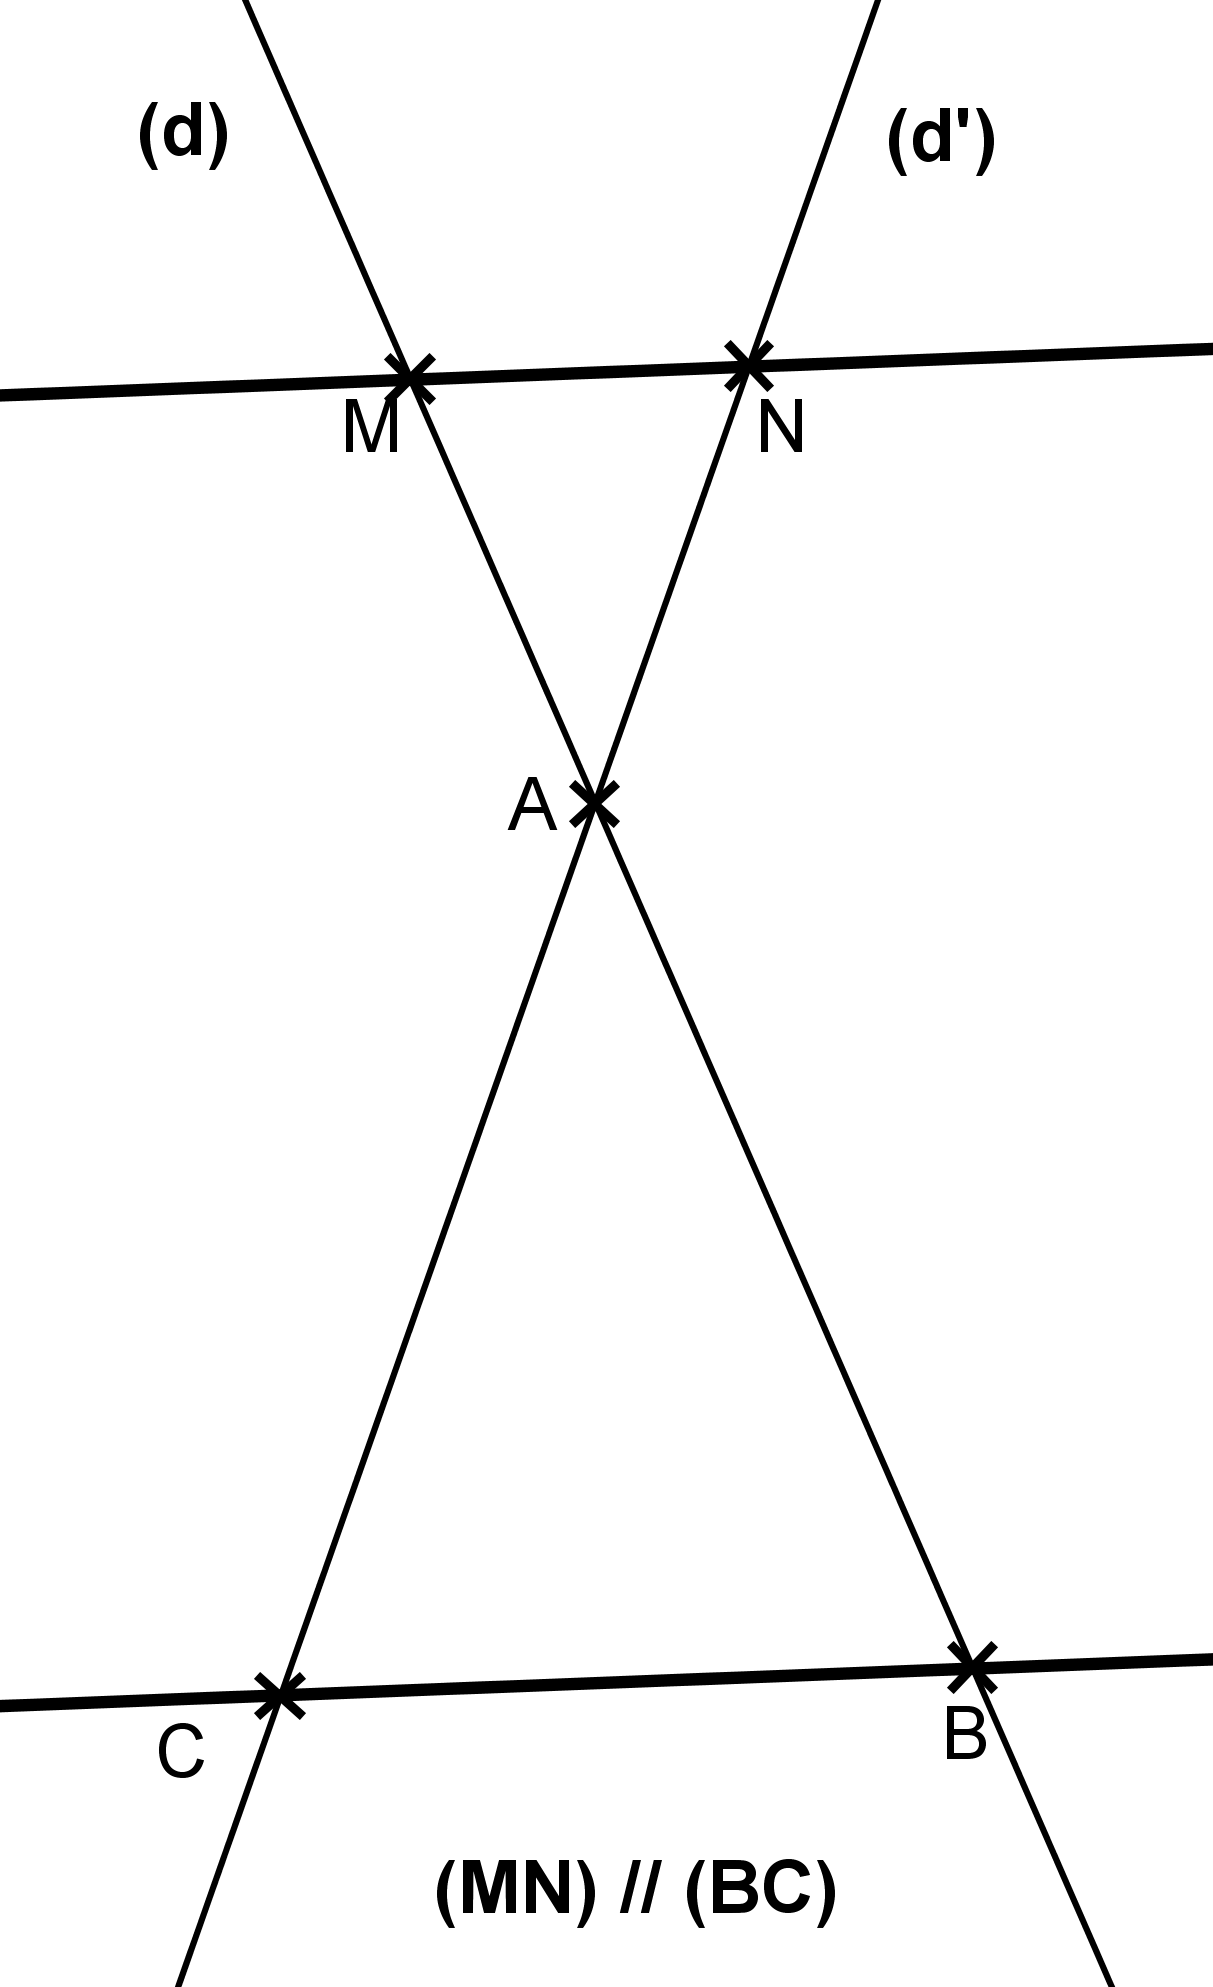
\includegraphics[width=4cm]{images/ex3.png}
\end{center}
\end{minipage}
\end{tabular}

\vspace{3cm}

\ul{Figures-cl�s}:


\begin{tabular}{ccc}
\begin{minipage}{6cm}
\begin{center}
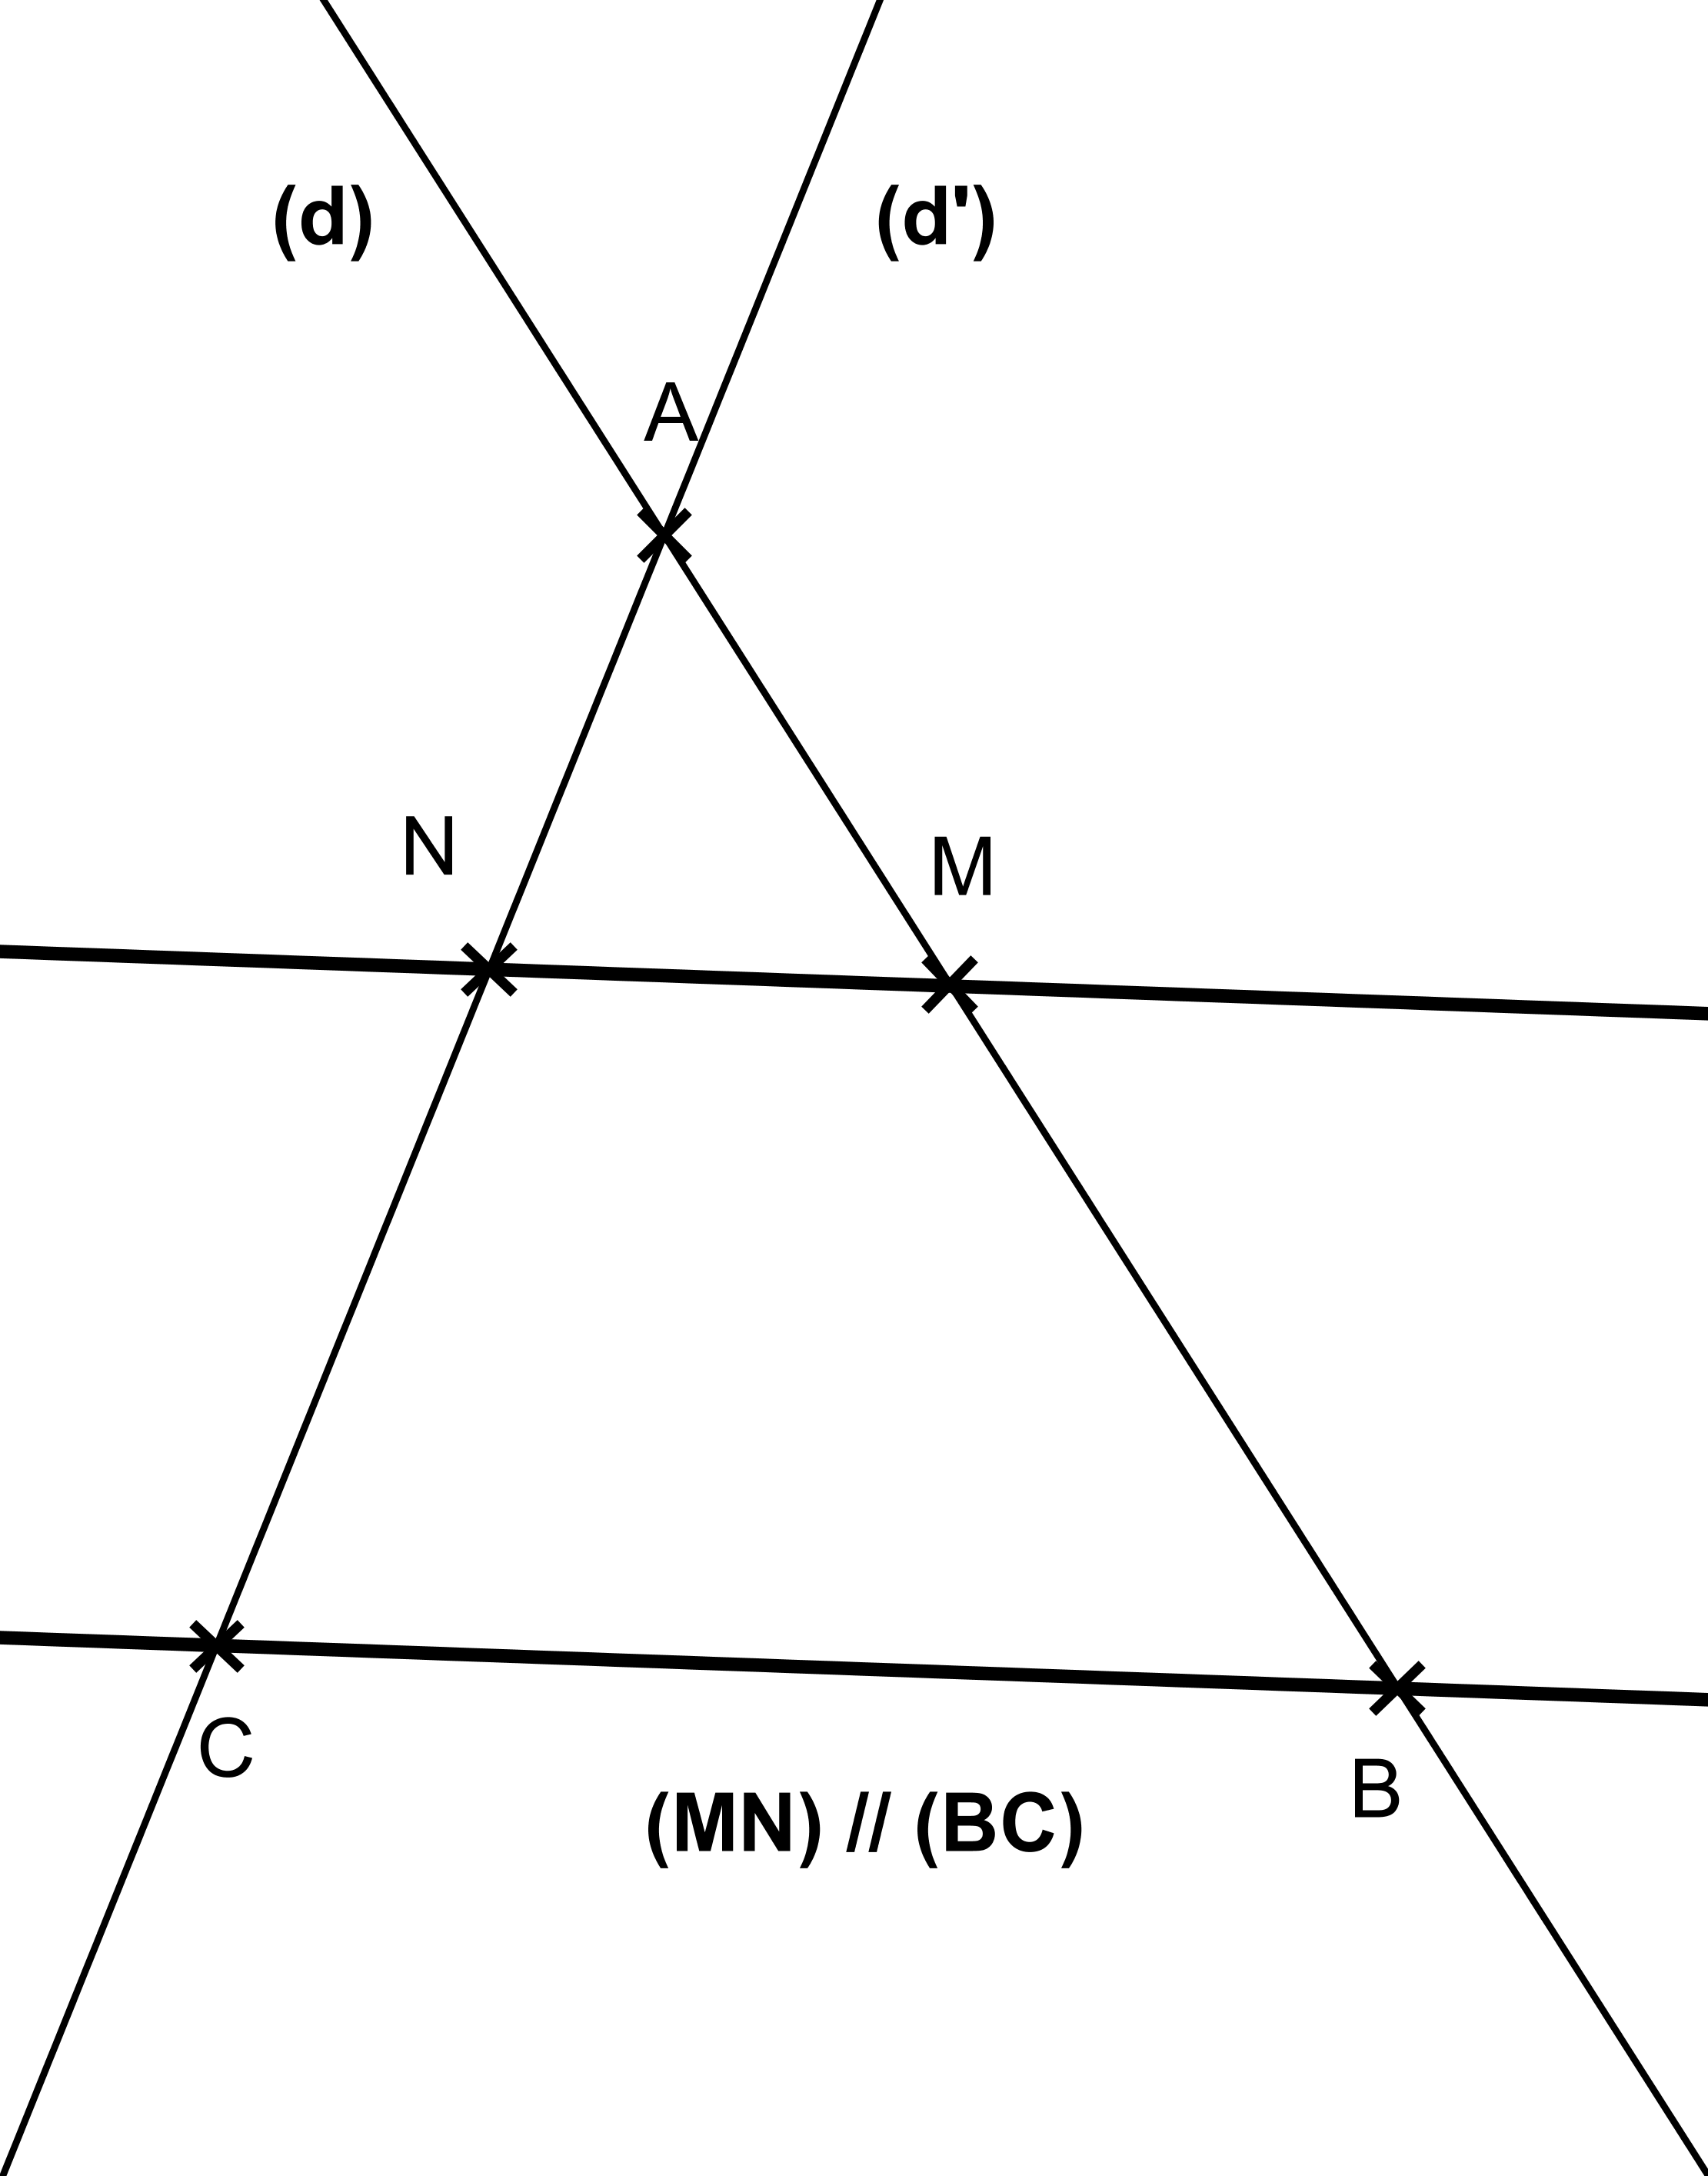
\includegraphics[width=5cm]{images/ex1.png}
\end{center}
\end{minipage}
&
\begin{minipage}{6cm}
\begin{center}
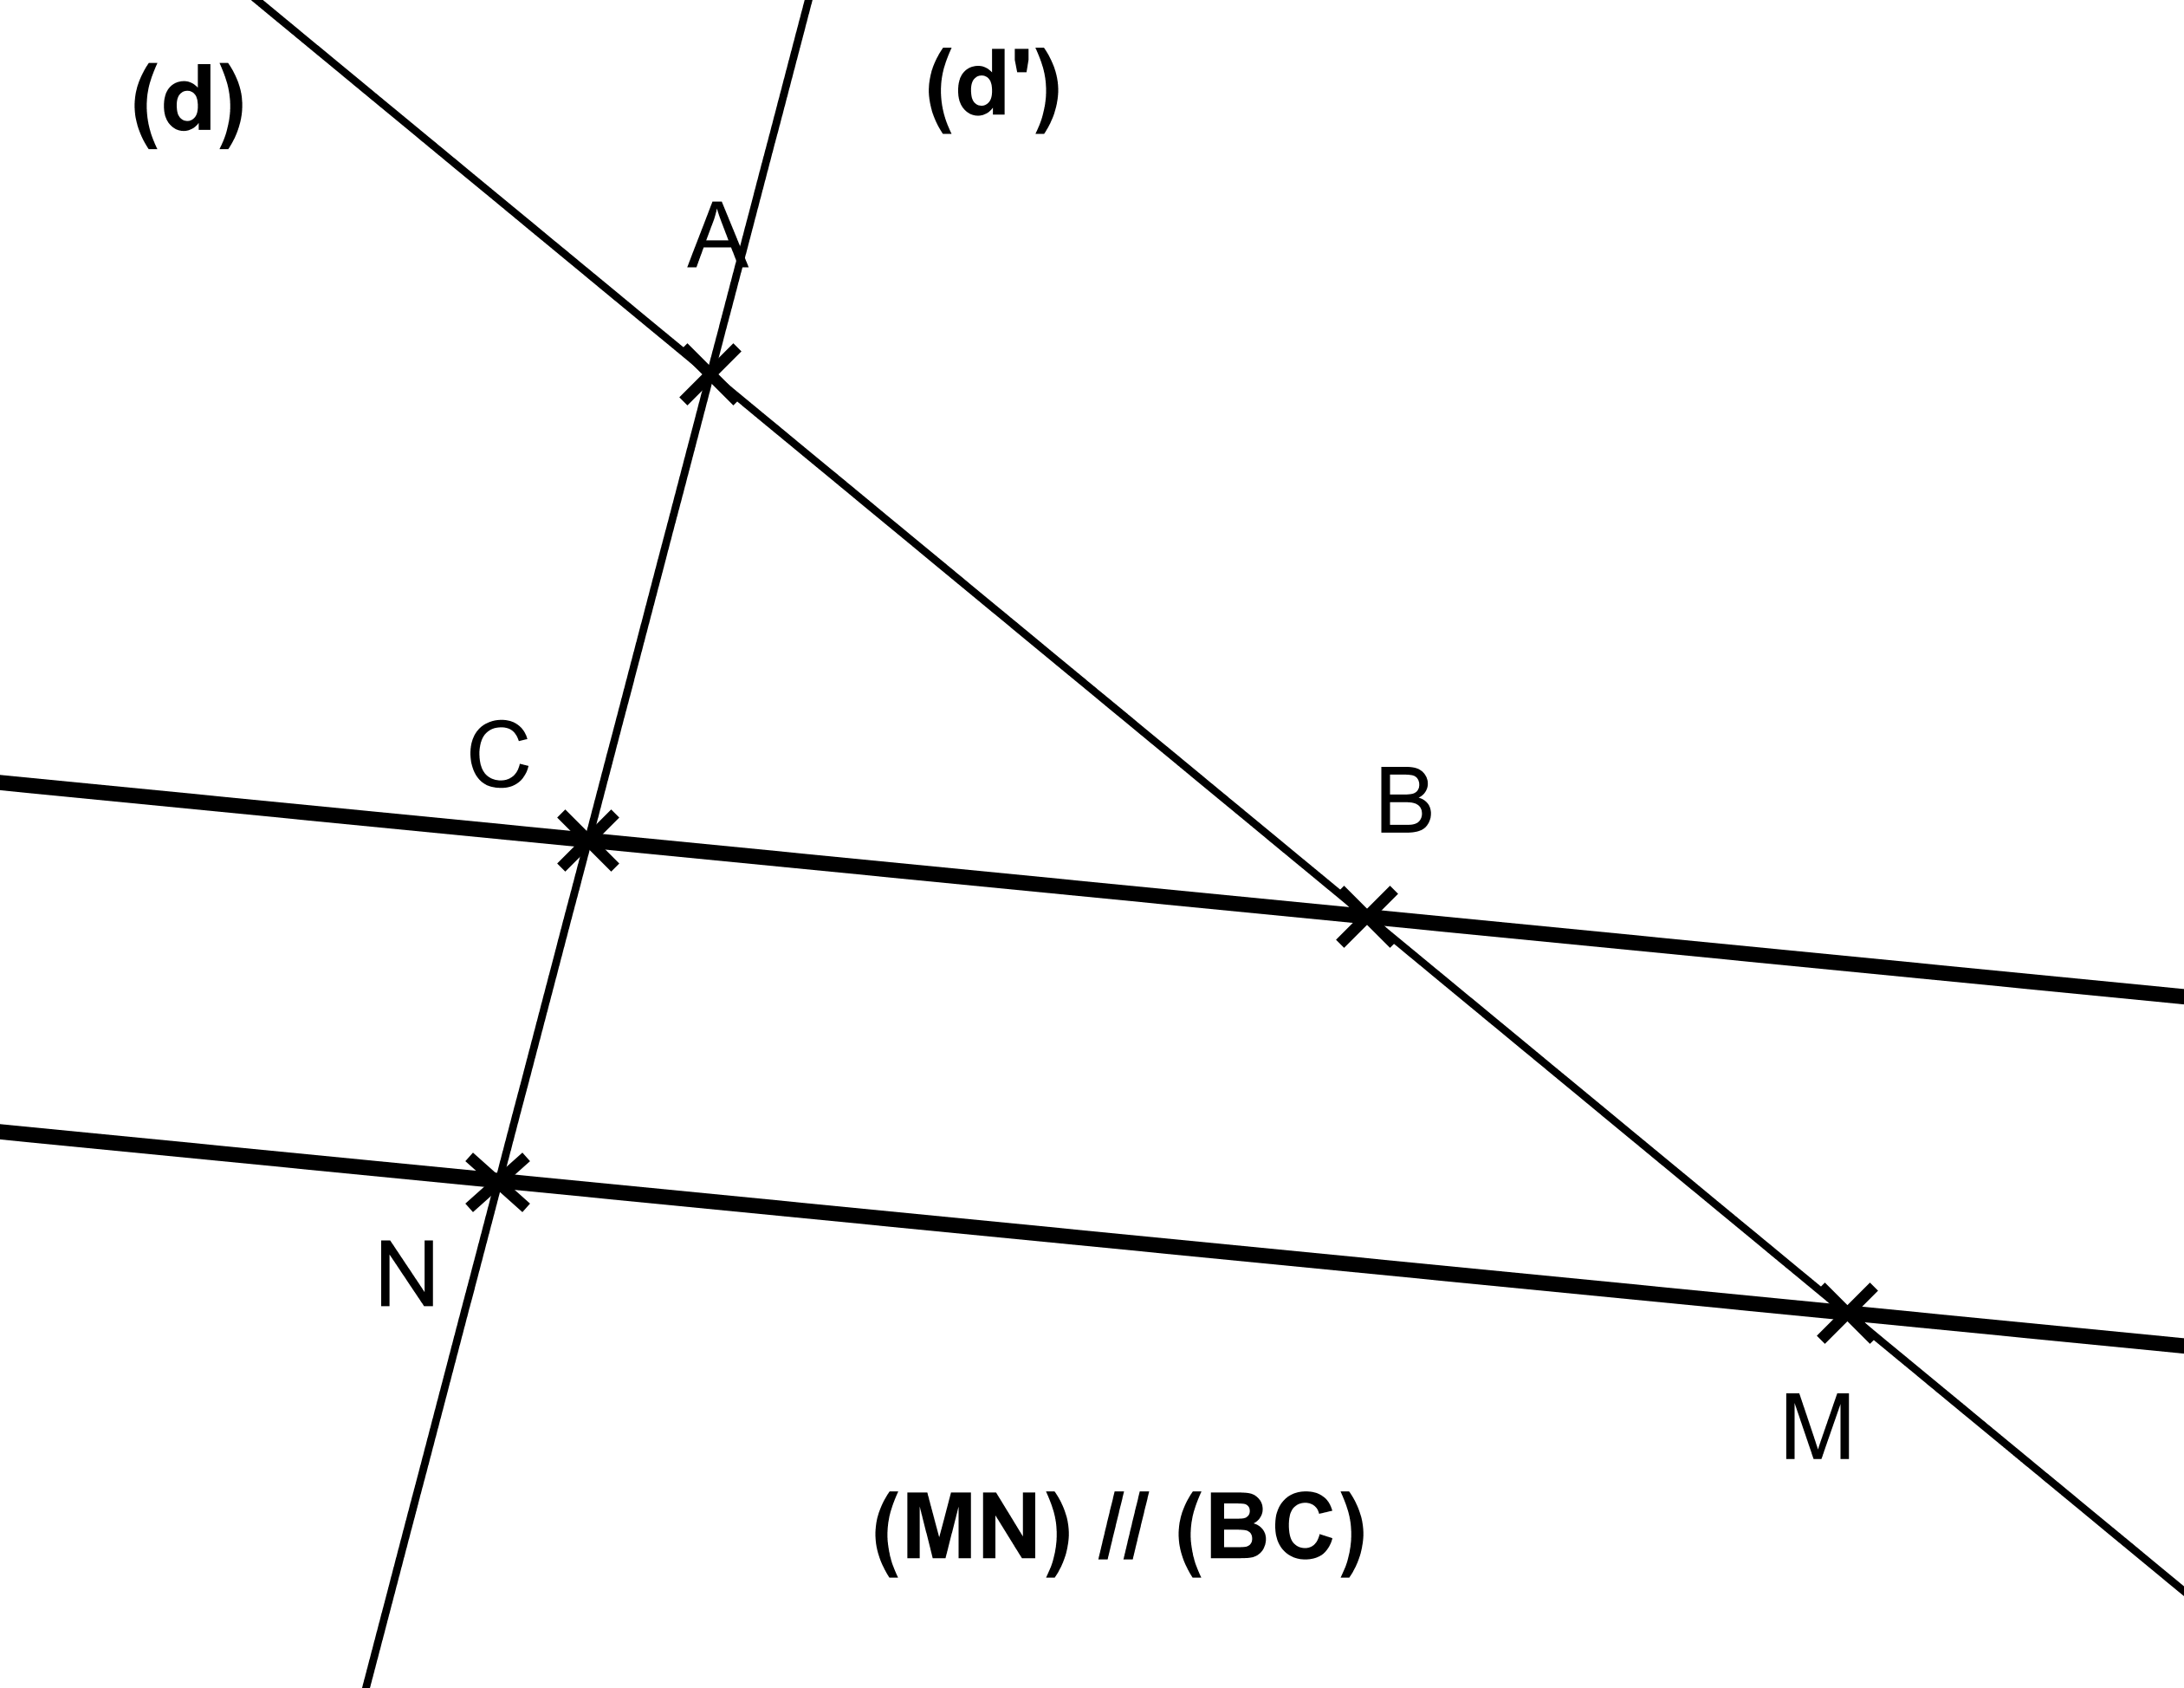
\includegraphics[width=5cm]{images/ex2.png}
\end{center}
\end{minipage}
& 
\begin{minipage}{6cm}
\begin{center}
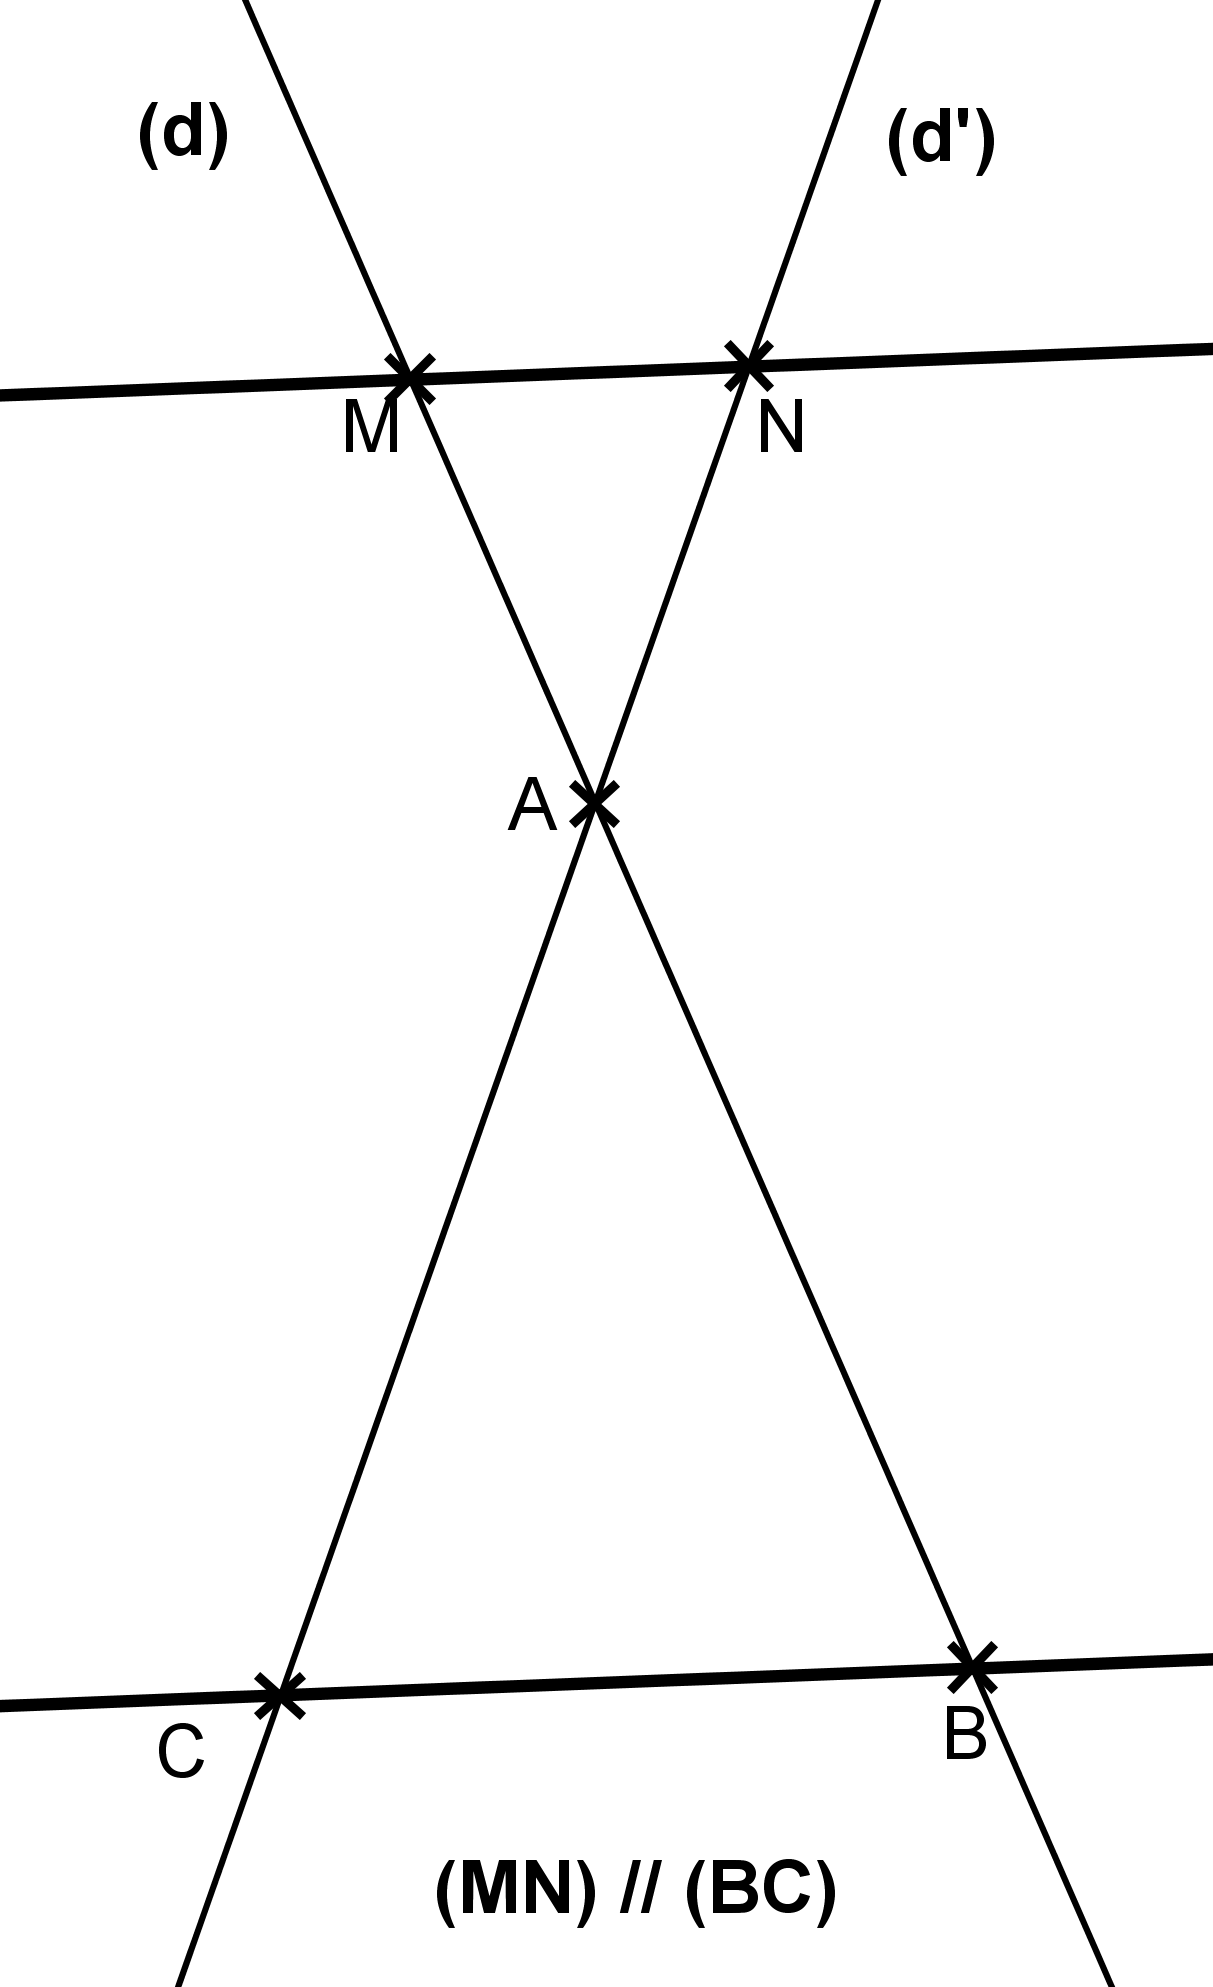
\includegraphics[width=4cm]{images/ex3.png}
\end{center}
\end{minipage}
\end{tabular}
\end{document}
